%%%%%%%%%%%%%%%%%%%%%%%%%%%%%%%%%%%%%%%%%
% Masters/Doctoral Thesis 
% LaTeX Template
% Version 1.41 (9/9/13)
%
% This template has been downloaded from:
% http://www.latextemplates.com
%
% Original authors:
% Steven Gunn 
% http://users.ecs.soton.ac.uk/srg/softwaretools/document/templates/
% and
% Sunil Patel
% http://www.sunilpatel.co.uk/thesis-template/
%
% License:
% CC BY-NC-SA 3.0 (http://creativecommons.org/licenses/by-nc-sa/3.0/)
%
% Note:
% Make sure to edit document variables in the Thesis.cls file
%
%%%%%%%%%%%%%%%%%%%%%%%%%%%%%%%%%%%%%%%%%

%----------------------------------------------------------------------------------------
%	PACKAGES AND OTHER DOCUMENT CONFIGURATIONS
%----------------------------------------------------------------------------------------

\documentclass[11pt, a4paper, twoside]{Thesis} % Paper size, default font size and one-sided paper

\graphicspath{{Pictures/}} % Specifies the directory where pictures are stored

\usepackage[square, numbers, comma, sort&compress]{natbib} % Use the natbib reference package - read up on this to edit the reference style; if you want text (e.g. Smith et al., 2012) for the in-text references (instead of numbers), remove 'numbers' 
\hypersetup{urlcolor=black, colorlinks=false} % Colors hyperlinks in blue - change to black if annoying
\title{\ttitle} % Defines the thesis title - don't touch this

\usepackage{amsmath}
\usepackage{microtype}	% Font improvement for pdflatex.
\usepackage{pgf}
\usepackage{tikz}
\usetikzlibrary{shapes,arrows}
\usepackage{verbatim}
\usepackage{url}
\usepackage{float}					% Floating figure placement.
\usepackage{multirow}
\usepackage{subfigure}
\usepackage{makeidx}
%\usepackage{IEEEtrantools}

% Listings for wrapping code.
\lstset{breaklines=true, basicstyle=\footnotesize\ttfamily, tabsize=4, numbers=left, stepnumber=1, frame=single, showstringspaces=false}
% Use this before inserting C++ code snippet using lstlisting.
\lstset{language=[ISO]C++, commentstyle=\color{green!50!black}, keywordstyle=\color{blue}, stringstyle=\color{red!60!black}}
% Use this before inserting Matlab code.
\lstset{language=Matlab, commentstyle=\color{green!50!black}, keywordstyle=\color{blue}, stringstyle=\color{red!60!black}}

% Links direct to top of figures.
\usepackage[all]{hypcap}

% Index directive.
\makeindex

% Line spacing.
\def\SingleSpacing{\def\baselinestretch{1}\large\normalsize}
\def\DoubleSpacing{\def\baselinestretch{1.5}\large\normalsize}

\tikzstyle{decision} = [diamond, draw, fill=yellow!20, 
    text width=5em, text badly centered, node distance=3cm, inner sep=0pt]
\tikzstyle{block} = [rectangle, draw, fill=blue!20, 
    text width=20em, text centered, rounded corners, minimum height=4em]
\tikzstyle{line} = [draw, -latex']
\tikzstyle{cloud} = [draw, ellipse,fill=red!20, node distance=3cm,
    minimum height=2em]
    
\let\Chaptermark\chaptermark
\def\chaptermark#1{\def\Chaptername{#1}\Chaptermark{#1}}
\let\Sectionmark\sectionmark
\def\sectionmark#1{\def\Sectionname{#1}\Sectionmark{#1}}

\setlength{\oddsidemargin}{1.5in}
\setlength{\evensidemargin}{1.5in}

\begin{document}

\frontmatter % Use roman page numbering style (i, ii, iii, iv...) for the pre-content pages

\setstretch{1.5} % Line spacing of 1.3

% Define the page headers using the FancyHdr package and set up for one-sided printing
\fancyhead{} % Clears all page headers and footers
\fancyhead[RO]{~\hfill\thepage}
\fancyhead[LE]{\thepage}
%\rhead{\thepage} % Sets the right side header to show the page number
%\lhead{} % Clears the left side page header

\pagestyle{fancy} % Finally, use the "fancy" page style to implement the FancyHdr headers

\newcommand{\HRule}{\rule{\linewidth}{0.5mm}} % New command to make the lines in the title page

% PDF meta-data
\hypersetup{pdftitle={\ttitle}}
\hypersetup{pdfsubject=\subjectname}
\hypersetup{pdfauthor=\authornames}
\hypersetup{pdfkeywords=\keywordnames}

%----------------------------------------------------------------------------------------
%	TITLE PAGE
%----------------------------------------------------------------------------------------

% Title page

\begin{titlepage}
\begin{center}

\textsc{\LARGE \univname}\\[0.5cm] % University name
% Project title.
\rule{\linewidth}{0.5mm}\\[0.3cm]
{\Large \bfseries \ttitle}\\
\rule{\linewidth}{0.5mm}\\[0.5cm]

{\large By}\\[0.2cm]
{\large \bfseries \ M. Junaid Nasir}\\[1.5cm]


{\large Supervised By}\\[0.2cm]
{\large \bfseries \ Engr. Attique Dawood}\\[1.9cm]



\includegraphics[scale=0.15]{Figures/NU_Logo.png}\\[0.8cm]

{\large \bfseries Department of Electrical Engineering}\\[0.2cm]
{\large \bfseries NUCES--FAST}\\[0.2cm]
{\large \bfseries ISLAMABAD, PAKISTAN}\\[0.2cm]
{\large \bfseries \today}

\end{center}
\end{titlepage}


%----------------------------------------------------------------------------------------
%	Developer's Submission
%----------------------------------------------------------------------------------------

\begin{center}


{\large This report is being submitted to the Department of Electrical Engineering of the National University of Computer and Emerging Sciences in partial fulfillment of the requirements for the degree of BS in Electrical Engineering}\\[0.5cm]
\end{center}


%----------------------------------------------------------------------------------------
%	DECLARATION PAGE
%----------------------------------------------------------------------------------------

\clearpage
\setstretch{1.2}
\Declaration{

\addtocontents{toc}{\vspace{1em}} % Add a gap in the Contents, for aesthetics

We take full responsibility of the project work conducted during the Final Year Project (FYP) titled { \bfseries \emph{``\ttitle''}}.We solemnly declare that the project work presented in the FYP report is done solely by us with no significant help from any other person; however, small help wherever taken is duly acknowledged.  We have also written the complete FYP report by ourselves. Moreover, we have not presented this FYP (or substantially similar project work) or any part of the thesis previously to any other degree awarding institution within Pakistan or abroad.

We understand that the management of Department of Electrical Engineering of National University of Computer and Emerging Sciences has a zero tolerance policy towards plagiarism. Therefore, we as an author of the above-mentioned FYP report solemnly declare that no portion of our report has been plagiarized and any material used in the report from other sources is properly referenced. Moreover, the report does not contain any literal citing of more than 70 words (total) even by giving a reference unless we have obtained the written permission of the publisher to do so. Furthermore, the work presented in the report is our own work and we have positively cited the related work of the other projects by clearly differentiating our work from their relevant work. 

We further understand that if we are found guilty of any form of plagiarism in our FYP report even after our graduation, the University reserves the right to withdraw our BS degree.  Moreover, the University will also have the right to publish our names on its website that keeps a record of the students who committed plagiarism in their FYP reports.”
\begin{flushright}
\rule{5cm}{0.2mm}\\
M. Junaid Nasir (10-0361)\\[0.8cm]
\rule{5cm}{0.2mm}\\
\hspace{1.8cm}
Certified by Supervisor\\[0.8cm]
\rule{5cm}{0.2mm}\\
Verified by Plagiarism Cell Officer\\[0.5cm]
Dated:~\rule{4.5cm}{0.2mm}\\[0.2cm]
\end{flushright}
}

\clearpage % Start a new page


%----------------------------------------------------------------------------------------
%	ABSTRACT PAGE
%----------------------------------------------------------------------------------------
%\vspace{3.5cm}
\addtotoc{Abstract} % Add the "Abstract" page entry to the Contents
\setstretch{1.5}
\abstract{\addtocontents{toc}{\vspace{1em}} % Add a gap in the Contents, for aesthetics

Negative Index Materials (NIM) is a hot research area having several
applications for example SuperLense, Fiber optics, RADAR systems, and Invisibility clocking. 
However, to model these applications using NIM is not an easy task, it requires complex algorithms
and considerable amount of time to simulate these objects. The aim of this project
is to provide a platform for future research in this field by implementing Finite Difference Time Domain (FDTD)
 algorithm for NIM and optimizing the program for less computational time using Graphics Process Unit (GPU).
In this project a NIM slab is modeled using the (frequency dependent dispersive) Drude model that have 
 refractive index of -1 (choosing $\mu_{r} = -1$ and $\epsilon_{r} = -1$ ) at 3 GHz

}

\clearpage % Start a new page

%----------------------------------------------------------------------------------------
%	ACKNOWLEDGEMENTS
%----------------------------------------------------------------------------------------

\setstretch{1.5} % Reset the line-spacing to 1.3 for body text (if it has changed)

\acknowledgements{\addtocontents{toc}{\vspace{1em}} % Add a gap in the Contents, for aesthetics

I would like to express my sincere gratitude to my supervisor Mr. Attique Dawood for the continuous support during my projct, for his  motivation, enthusiasm, and immense knowledge. His guidance helped me in all the time of FYP and writing of this thesis. I also take this opportunity to express a deep sense of gratitude to my co-supervisor Ms. Hina Ashraf, for her cordial support, valuable information and guidance. Her willingness to motivate me contributed tremendously to this project.

}
\clearpage % Start a new page

%----------------------------------------------------------------------------------------
%	LIST OF CONTENTS/FIGURES/TABLES PAGES
%----------------------------------------------------------------------------------------

\pagestyle{fancy} % The page style headers have been "empty" all this time, now use the "fancy" headers as defined before to bring them back

\lhead{\emph{Table of Contents}} % Set the left side page header to "Contents"
\tableofcontents % Write out the Table of Contents

\lhead{\emph{List of Figures}} % Set the left side page header to "List of Figures"
\listoffigures % Write out the List of Figures

%\lhead{\emph{List of Tables}} % Set the left side page header to "List of Tables"
%\listoftables % Write out the List of Tables

%----------------------------------------------------------------------------------------
%	ABBREVIATIONS
%----------------------------------------------------------------------------------------

\clearpage % Start a new page

\setstretch{1.5} % Set the line spacing to 1.5, this makes the following tables easier to read

\lhead{\emph{Abbreviations}} % Set the left side page header to "Abbreviations"
\listofsymbols{ll} % Include a list of Abbreviations (a table of two columns)
{
\textbf{NIM} & \textbf{N}egtive \textbf{I}ndex \textbf{M}aterial \\
\textbf{LHM} & \textbf{L}eft \textbf{H}anded \textbf{M}aterial \\
\textbf{DNG} & \textbf{D}ouble \textbf{N}e\textbf{G}ative (Material) \\
\textbf{EM} & \textbf{E}lectrico\textbf{M}agnetic\\
\textbf{FDTD} & \textbf{F}inite \textbf{D}ifference \textbf{T}ime \textbf{D}omain \\
\textbf{GPU} & \textbf{G}raphical \textbf{P}rocessing \textbf{U}nit \\
\textbf{OpenCL} & Open \textbf{C}omputing \textbf{L}anguage \\
\textbf{AMD} & \textbf{A}dvance \textbf{M}icro \textbf{D}evices \\
\textbf{PMC} & \textbf{P}erfect \textbf{M}agnetic \textbf{C}onductor \\
\textbf{ABC} & \textbf{A}bsorbing \textbf{B}oundary \textbf{C}ondition \\
%\textbf{Acronym} & \textbf{W}hat (it) \textbf{S}tands \textbf{F}or \\
}

%----------------------------------------------------------------------------------------
%	PHYSICAL CONSTANTS/OTHER DEFINITIONS
%----------------------------------------------------------------------------------------

%\clearpage % Start a new page

%\lhead{\emph{Physical Constants}} % Set the left side page header to "Physical Constants"

%\listofconstants{lrcl} % Include a list of Physical Constants (a four column table)
%{
%Speed of Light & $c$ & $=$ & $2.997\ 924\ 58\times10^{8}\ \mbox{ms}^{-\mbox{s}}$ (exact)\\
% Constant Name & Symbol & = & Constant Value (with units) \\
%}


%----------------------------------------------------------------------------------------
%	THESIS CONTENT - CHAPTERS
%----------------------------------------------------------------------------------------
\mainmatter % Begin numeric (1,2,3...) page numbering

\pagestyle{fancy} % Return the page headers back to the "fancy" style
\fancyhead{} % Clears all page headers and footers
%\lhead[\rm\thepage]{\fancyplain{}{\sl{\rightmark}}}
%\rhead[\fancyplain{}{\sl{\leftmark}}]{\rm\thepage}
\lhead{}
\rhead{}
\fancyhead[RO]{\thechapter\hfill\thepage}
\fancyhead[LE]{\thepage\hfill\Sectionmark}
% Include the chapters of the thesis as separate files from the Chapters folder
% Uncomment the lines as you write the chapters

% Chapter Template

\chapter{Introduction} % Main chapter title

\label{Chapter1} % Change X to a consecutive number; for referencing this chapter elsewhere, use \ref{ChapterX}

\fancyhead[RO]{\thepage}
\fancyhead[RE]{\thepage}
\fancyhead[LE]{Chapter 1.~\emph{\Chaptername}}
\fancyhead[LO]{\emph{\ttitle}}

%----------------------------------------------------------------------------------------
%	SECTION 1
%----------------------------------------------------------------------------------------

\section{Background }
\index{NIM}
In 2000 Smith, Schultz and coworkers \cite{smith} demonstrated that it is possible to create a material artificially to have different EM  characteristics, it was the first NIM ever created. Negative Index Material (NIM) or Left Handed Material (LHM) is a material which has negative permeability and permittivity. Due to this it behaves differently as compared to naturally occurring materials. Although NIM have been introduced in 1968 \cite{vesel}
it's surprising phenomena are still not well understood in details.

 In addition
to a negative index (NI) of refraction, properties such as artificial
magnetism \cite{pendry}
, negative permittivity, and negative permeability have
been observed in fabricated NIM composites; 
Having these special characteristics NIM became ideal candidate 
for applications like Super Lens, Optical fiber cable, RADAR systems, EM absorbers.and invisibility cloaking. With
encouraging results having been demonstrated at microwave
frequencies, there has been a determined push to extend NIMs to
the terahertz, infrared, and visible bands which resulted in establishment of many
research programs, conferences, workshops, and significant
funding efforts dedicated to understanding and developing NIMs.
Since 2000, the rate of publications on EM-NIMs has grown
exponentially, \cite{rama}
indicating the increase in interest that NI
materials have generated. Much of that interest has been sparked by
the property of negative refractive index.

\begin{figure}[htbp]
	\centering
		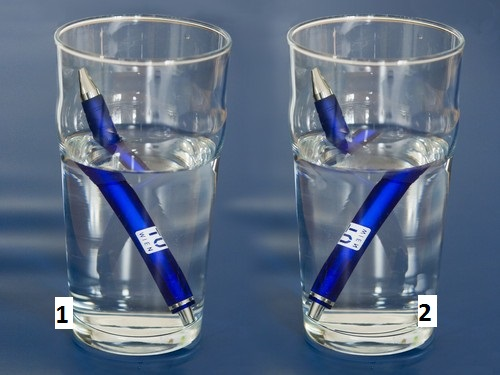
\includegraphics[width=4in]{Pictures/glass.jpg}
		\rule{35em}{0.5pt}
	\caption[Illustration of NIM]{(1) shows the normal phenomenon of refraction in water having positive value of refractive index. (2) shows the unusual phenomenon of refraction in water having negative value of refractive index}
	\label{fig:glass}
\end{figure}


%----------------------------------------------------------------------------------------
%	SECTION 2
%----------------------------------------------------------------------------------------
\index{Problem statement}
\section{Problem Statement}

To model an NIM (slab) using (frequency dependent dispersive) drude model that will effectively have refractive index of -1 (choosing $\mu_{r} = -1$ and $\epsilon_{r} = -1$ ) at 3 GHz.

Objectives of this project are 
\begin{itemize}
\item[-] To simulate and observe the behavior of Electromagnetic Waves when they pass through negative index materials
\item[-] To use FDTD algorithm and modify it for negative index material simulations
\item[-] Reducing computational time by using the parallel processing power of Graphics Processing Units (GPU)
\item[-] Comparison of algorithm performance on different platforms (MATLAB, C++, GPU)
\end{itemize}

%-----------------------------------
%	SUBSECTION 1
%-----------------------------------
%\subsection{Negative Index Material}


% Chapter Template

\chapter{Design and Implementation} % Main chapter title

\label{Chapter2} % Change X to a consecutive number; for referencing this chapter elsewhere, use \ref{ChapterX}

%\lhead{Chapter 2. \emph{Design and Implementation}} % Change X to a consecutive number; this is for the header on each page - perhaps a shortened title
\fancyhead[RO]{\thepage}
\fancyhead[RE]{\thepage}
\fancyhead[LE]{Chapter 2.~\emph{\Chaptername}}
\fancyhead[LO]{\emph{\ttitle}}
%----------------------------------------------------------------------------------------
%	SECTION 1
%----------------------------------------------------------------------------------------

\section{Modeling of a denser slab}

A denser slab having $\mu_r = 2\mu_o$ and $\epsilon_r = 2\epsilon_o$
is simulated to test the results and accuracy of our algorithm. these results will be compared with
results of NIM slab.

%-----------------------------------
%	SUBSECTION 1.1
%-----------------------------------
\subsection{Finite Difference Time Domain (FDTD) technique}
\index{Finite Difference Time Domain (FDTD) technique}
FDTD method is used to solve problems related to electromagnetic. It is very easy to implement but require much computational power and time as this is a recursive technique. The main benefit of using this technique is that it is accurate on wide range of frequency. 

Maxwell's equations (Ampere's and Faraday's laws) can be written as finite differences using FDTD. A function $f(x)$ whose value need to be found at $x_o$ is given by \eqref{fxwali}
	\begin{equation}
	\left. \frac {df(x)}{d(x)}\right|_{x=x_o} \approx 
	\frac {f \left( x_o + \frac{\delta}{2} \right) - f \left( x_o - \frac{\delta}{2} \right) }{\delta}
	\label{fxwali}
	\end{equation}
this equation provides an approximation of derivative of $f(x)$ at $x_o$ but the function is sampled at an offset $\delta$ from the original point $x_o$. It have second-order accuracy or second-order behavior. This implies if $\delta$ is reduced by a factor of 10 the error will be reduced by 100. if $\delta = 0$ then $error = 0$.
%-----------------------------------
%	SUBSECTION 1.2
%-----------------------------------
\subsection{The Yee Algorithm}
\index{Kane Yee}
Kane Yee proposed FDTD algorithm in 1966\cite{kane}
. It can be summarized as follows:
\begin{enumerate}
\item Differential forms of Maxwell's equations are written with finite differences.
\item Solve the difference equations to get "update equations" that express the future value in terms of past value. Figure \ref{fig:fdtd}
\begin{figure}[htbp]
	\centering
		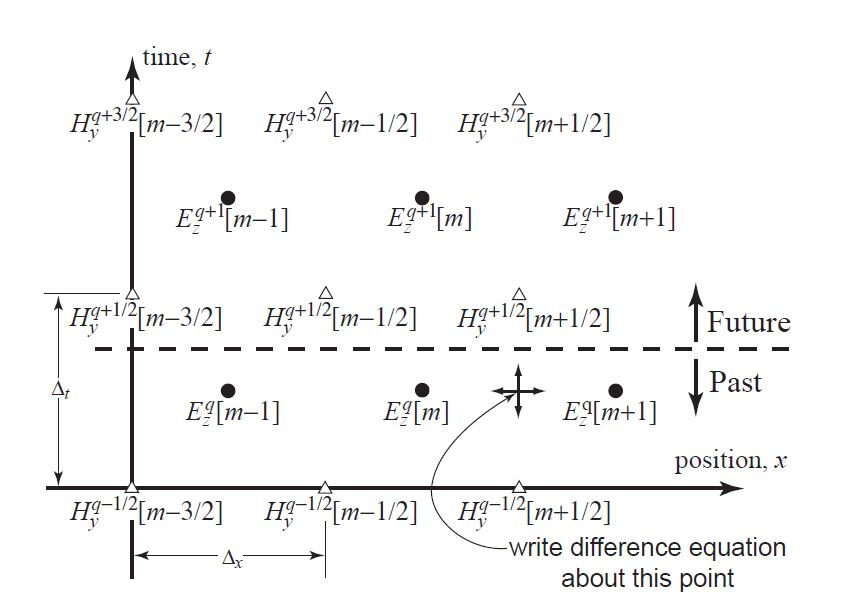
\includegraphics[width=4in]{Pictures/fdtd.jpg}
		%\rule{35em}{0.5pt}
	\caption[FDTD update equations]{Update equations at a point depend on past values of adjacent points.}
	\label{fig:fdtd}
\end{figure} 
\item Find the magnetic field component one time-step into the future for complete spatial domain. Using equation \eqref{eq:mag}
\begin{equation}
	H_y^{q+\frac {1}{2}} \left[ m + \frac {1}{2} \right] = H_y^{q-\frac {1}{2}} \left[ m + \frac {1}{2} \right]
+ \frac {\Delta_t}{\mu\Delta_x} \left( E_z^q \left[ m+1 \right] - E_z^q \left[m\right] \right)
\label{eq:mag}
\end{equation}
\item Find the electric field component one time-step into the future for complete spatial domain. Using equation \eqref{eq:ele}
\begin{equation}
 E_z^{q+1} \left[m\right] =  E_z^q \left[m\right] + \frac {\Delta_t}{\epsilon\Delta_x}  \left( H_y^{q+\frac {1}{2}} \left[ m + \frac {1}{2} \right] - H_y^{q+\frac {1}{2}} \left[ m - \frac {1}{2} \right]  \right)
\label{eq:ele}
\end{equation}
\item Repeat step 4 and 5 until the desired duration of time.
\end{enumerate}

The equations \eqref{eq:mag} and \eqref{eq:ele} does not relate to how far energy can propagate in one time step. The maximum speed at at which energy can travel is speed of light $c = \frac {1}{\sqrt\epsilon_o\mu_o}$ hence the maximum distance is $c\Delta_t$. An important factor is Courant number $S_c =  \frac {c\Delta_t}{\Delta_x}$ which relates the maximum distance with that of distance traveled by the energy under study. The coefficients in equations \eqref{eq:mag} and \eqref{eq:ele} can be written as 
\begin{equation}
	\frac {\Delta_t}{\epsilon\Delta_x} = \frac {\eta_0}{\epsilon_r}S_c
\end{equation}
\begin{equation}
	\frac {\Delta_t}{\mu\Delta_x} = \frac {1}{\mu_r\eta_0}S_c
\end{equation}
where $\eta-0 = \sqrt\mu_0\epsilon_0$ is impedance of free space.

\begin{figure}[htbp]
	\centering
		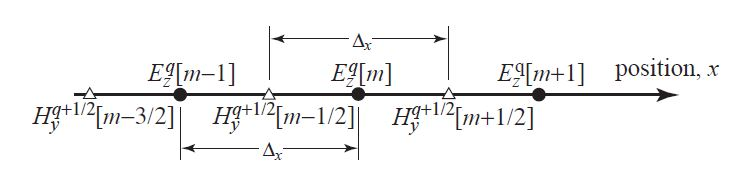
\includegraphics[width=4in]{Pictures/1dfdtd.jpg}
		%\rule{35em}{0.5pt}
	\caption[1 dimensional FDTD Space]{A one-dimensional FDTD space showing the spatial offset between magnetic and electric fields.}
	\label{fig:1dfdtd}
\end{figure} 

%-----------------------------------
%	SUBSECTION 1.3
%-----------------------------------
\subsection{One-Dimensional FDTD simulation}
To simulate  equations \eqref{eq:mag} and \eqref{eq:ele} in MATLAB we have to keep in mind following things:
MATLAB uses integer numbers for indexes of arrays hence we use does not set an offset of $\frac{1}{2}$ instead we use same integers for indexes as well, Figure \ref{fig:fdtdpc} shows a graphical representation of FDTD algorithm with integer indexes
\begin{figure}[htbp]
	\centering
		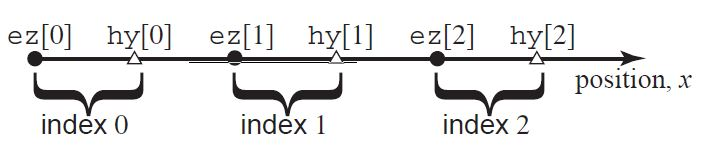
\includegraphics[width=5in]{Pictures/fdtdpc.jpg}
		%\rule{35em}{0.5pt}
	\caption[1 dimensional FDTD Space assumed with integer indices]{A one-dimensional FDTD space showing the assumed indexes and locations of magnetic and electric component in spatial domain}
	\label{fig:fdtdpc}
\end{figure}
Keeping figure \ref{fig:fdtdpc} in mind, the two update equations become
\lstset{language=Matlab, commentstyle=\color{green!50!black}, keywordstyle=\color{blue}, stringstyle=\color{red!60!black}}
\begin{lstlisting}
for m=0:SIZE-1
	hy[m] = hy[m] + (ez[m + 1] - ez[m]) / imp0;
end
for m=1:SIZE
	ez[m] = ez[m] + (hy[m] - hy[m - 1])  * imp0;
end
\end{lstlisting}
where imp0 is impedance of free space.
The reason behind different loop start and end point is that at end nodes there are no neighboring nodes to one side. For example hy[-1] node for ez[0].
As the field is initially zero it will remain zero as there is no energy passing through it. to overcome this problem a source node is hard-coded into one of the entry of array 
\lstset{language=Matlab, commentstyle=\color{green!50!black}, keywordstyle=\color{blue}, stringstyle=\color{red!60!black}}
\begin{lstlisting}
	ez(1) = exp(-(qTime - 30) * (qTime - 30) / 100.); %update node hard-coded
\end{lstlisting}

\textbf{Results}\\
By using the program in Appendix \ref{matlab1}
we get the results in figure \ref{fig:fdtdpc}.
\begin{figure}[htbp]
	\centering
		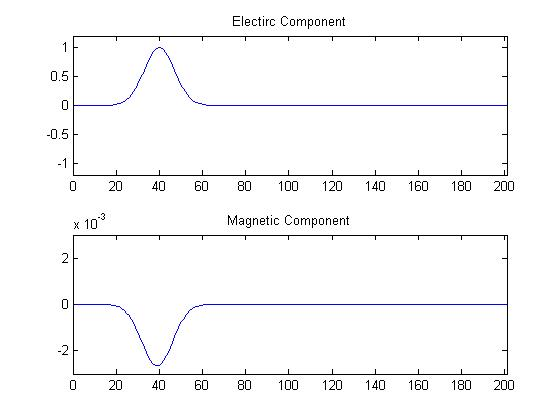
\includegraphics[width=5in]{Figures/free.jpg}
		%\rule{35em}{0.5pt}
	\caption[Simulation Result of 1 dimensional FDTD in free space]{Simulation Results of one-dimensional FDTD in free space showing both electric and magnetic component}
	\label{fig:fdtdpc}
\end{figure}
%-----------------------------------
%	SUBSECTION 1.4
%-----------------------------------
\subsection{Boundary Conditions}
\index{Grid truncation}
Grid termination is called boundary condition because there are no neighboring values at boundary. we must use some kind of boundary condition depending upon the requirements. two type of boundary conditions are mentioned below.
%-----------------------------------
%	SUBSECTION 1.4.1
%-----------------------------------
\subsubsection{Perfect Conductor Boundary}
In program Appendix \ref{matlab2}
grid is terminated with a zero value of magnetic field
making it a perfect magnetic conductor (PMC) which reflects the wave completely. it also inverts the magnetic component of the wave figure \ref{fig:pmc}. In reality PMC does not exists hence to make this simulation as close to real behavior we use some other method to truncate the grid.
\begin{figure}[htbp]
	\centering
		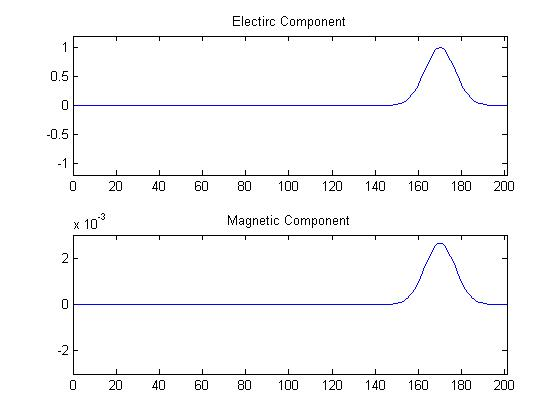
\includegraphics[width=5in]{Figures/pmc.jpg}
		%\rule{35em}{0.5pt}
	\caption[Simulation Result of 1 dimensional FDTD in free space with Perfect magnetic conductor boundary]{Simulation Results of one-dimensional FDTD after reflecting from Perfect magnetic conductor}
	\label{fig:pmc}
\end{figure}
%-----------------------------------
%	SUBSECTION 1.4.2
%-----------------------------------
\subsubsection{Absorbing Boundary Conditions}
\index{ABC}
Perfect conductor boundary depends on the speed of propagation. It requires that at each time instant the wave also propagate by one spatial step, but with the introduction of dielectric (slab) the speed of propagation decreases resulting in unstable simulation. hence we need an advance boundary condition which is differential equation based absorbing boundary condition (ABC).
\begin{equation}
	E_z^{q+1} \left[ 0 \right] = E_z^q \left[ 1 \right] + \frac {\frac{S_c}{\sqrt\mu_r\epsilon_r}-1} {\frac{S_c}{\sqrt\mu_r\epsilon_r}+1} \left( E_z^{q+1} \left[ 1 \right] - E_z^q \left[ 0 \right]  \right)
\label{abc222}
\end{equation}
Equation \eqref{abc222} is absorbing boundary equation
for electric field. As it can be seen that this boundary condition also depends upon last time step value at boundary point. so we need to save that value in our program as well.
Program in appendix \ref{matlab3}
implements this boundary condition.

\textbf{Results}\\
Figure \ref{fig:abc} shows Gaussian wave after passing through a denser slab with absorbing boundary condition
\begin{figure}[htbp]
	\centering
		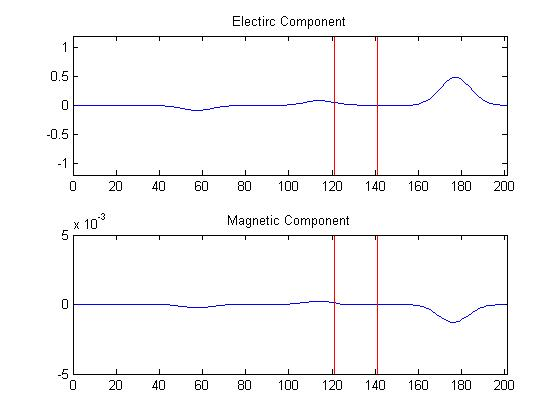
\includegraphics[width=5in]{Figures/abc.jpg}
		%\rule{35em}{0.5pt}
	\caption[Simulation Result of 1 dimensional FDTD after passing through denser medium]{Simulation Results of one-dimensional FDTD after passing through denser medium with absorbing boundary conditions}
	\label{fig:abc}
\end{figure}

%-----------------------------------
%	SUBSECTION 1.5
%-----------------------------------
\subsection{Simulation Results}
Following results were found after running program \ref{matlab4}
 this program implements FDTD algorithm in free space, denser medium slab, additive source and absorbing boundary conditions and perform post processing on simulation results.
%-----------------------------------
%	SUBSECTION 1.5.1
%-----------------------------------
\subsubsection{Simulation Parameters}
Parameters for program  \ref{matlab4}
are \\
Medium 1 = Free space  $\mu=\mu_0$  $\epsilon=\epsilon_0$\\
Medium 2 = slab of denser medium $\mu=2\mu_0$  $\epsilon=2\epsilon_0$\\
Courant Number $S_c=1$\\
Source type = Additive\\
Boundary conditions = Absorbing boundary conditions
%-----------------------------------
%	SUBSECTION 1.5.2
%-----------------------------------
\subsubsection{Frequency Domain Analysis}
\index{FDTD Frequency Analysis}
Frequency domain analysis compares the theoretical values with that of simulated values.
 In Frequency domain analysis spectrum of transmitted and Incident waves are plotted. 
Refractive index is also calculated which should be equal to calculated refractive index given by equation \eqref{refractiveindex}
\begin{equation}
	\eta=\sqrt\epsilon_r\mu_r
\label{refractiveindex}
\end{equation}
for medium having $\mu=2\mu_0$  $\epsilon=2\epsilon_0$ result of equation \eqref{refractiveindex} comes out to be 1.414

\begin{figure}[htbp]
	\centering
		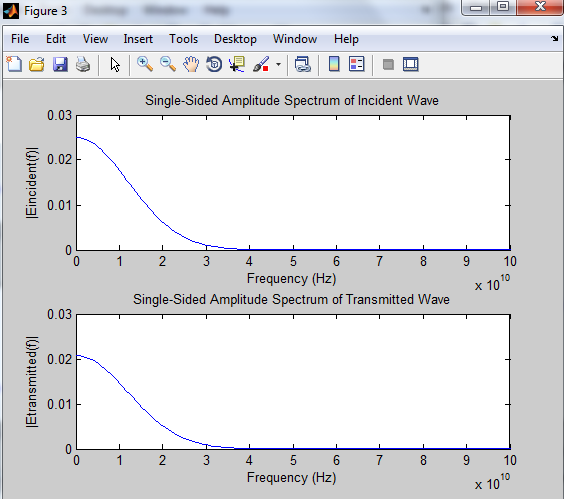
\includegraphics[width=5in]{Figures/fft1.png}
		%\rule{35em}{0.5pt}
	\caption[Frequency Spectrum of 1D denser medium slab]{Frequency Spectrum of transmitted and reflected wave after passing through a slab of denser medium having $\mu=2\mu_0$  $\epsilon=2\epsilon_0$ }
	\label{fig:fft1}
\end{figure}
\begin{figure}[htbp]
	\centering
		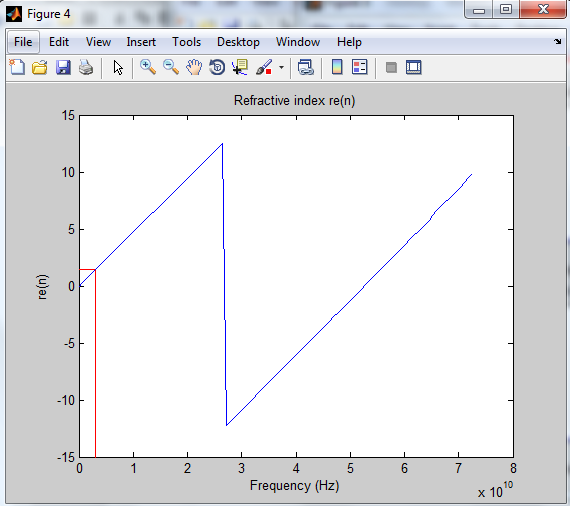
\includegraphics[width=5in]{Figures/ri1.png}
		%\rule{35em}{0.5pt}
	\caption[Refractive index of different frequencies after passing through denser medium]{Refractive index of different frequencies after passing through denser medium, Red lines shows the theoretical values of refractive index at 3Ghz Frequency}
	\label{fig:ri1}
\end{figure}
From figure \ref{fig:ri1} it is clear that simulation result and theoretical results are same as calculated from equation \eqref{refractiveindex}.
%-----------------------------------
%	SECTION 2
%-----------------------------------
\section{Modeling of NIM slab }
%-----------------------------------
%	SUBSECTION 2.1
%-----------------------------------
\subsection{Limitation of FDTD}
The standard FDTD does not work for negative values of permittivity and permeability. Reason behind this is Courant stability criterion. hence a NIM object can not be modeled using standard FDTD algorithm. Drude dispersive model or Lorentz model are used to implement NIM object. These models introduce frequency of operation $(\omega)$ into update equations.
%-----------------------------------
%	SUBSECTION 2.2
%-----------------------------------
\subsection{The Drudes Model}
\index{Drudes Model}
Ideally permeability and permittivity of a material remain constant for all values of operating frequencies. However in reality Speed of electromagnetic waves changes with frequency and there is also loss due to particle collisions inside material. A material is called dispersive if it's permeability or permittivity is frequency dependent.
Paual Drude proposed a model of transport properties in materials in 1990\citep{drude}.
\begin{equation}
	M\frac{d^2x}{dt^2} = QE(t) - Mg\frac{dx}{dt}
\label{drudee1}
\end{equation}
Equation \eqref{drudee1} is a Drude's 2nd order differential equation that relates to kinetic energy in moving charges under an electric field. The relative Permittivity in Drudes model is given by 
\begin{equation}
\hat{\epsilon_r} (w) = \epsilon_{\infty}- \frac{\omega_p^2}{\omega^2 - jg\omega}
\label{drudee2}
\end{equation}
setting $g=0$ and $ \epsilon_{\infty} = 1$ in equation \eqref{drudee2}, value of permittivity comes out to be negative for $\frac{\omega}{\omega_p} > 1$ (figure \ref{drude1})
\begin{figure}[htbp]
	\centering
		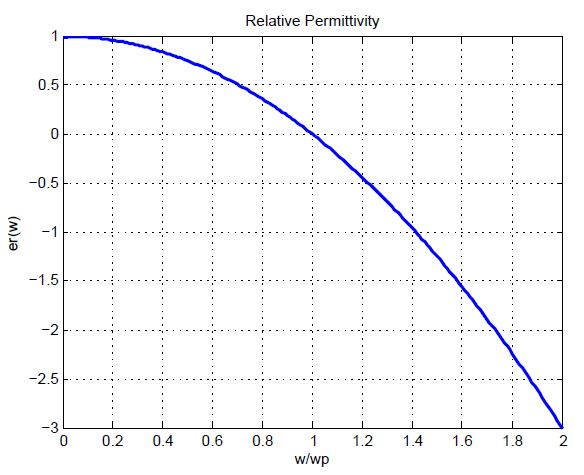
\includegraphics[width=5in]{Figures/drude1.jpg}
		%\rule{35em}{0.5pt}
	\caption[Permittivity in Drudes model for different frequencies]{Relative Permittivity plotted against $\frac{\omega}{\omega_p}$ for $g=0$ and $ \epsilon_{\infty} = 1$ }
	\label{drude1}
\end{figure}

%----------------------------------------------------------------------------------------
%	SUB SUB SECTION 2.2.1
%----------------------------------------------------------------------------------------

\subsubsection{Drudes Algorithm}
Auxiliary update equations for electric and magnetic components in Drudes model are give by \eqref{drudemag} and \eqref{drudeele}.
\begin{equation}
\begin{split}
	H_y^{n+1} &= a_m \left( B_y^{n+1} - 2B_y^n + B_y^{n-1} \right) + b_m \left( B_y^(n+1) - B_y^{n-1}  \right)\\
&+c_m \left( 2H_y^n-H_y^{n-1} \right) + d_m \left( 2H_y^n + H_y^{n-1} \right) +e_m H_y^{n-1}\\
\end{split}
\label{drudemag}
\end{equation}
\begin{equation}
\begin{split}
	E_z^{n+1} &= a_e \left( D_z^{n+1} - 2D_z^n + D_z^{n-1} \right) + b_e \left( D_z^(n+1) - D_z^{n-1}  \right)\\+ 
&c_e \left( 2E_z^n-E_z^{n-1} \right) + d_e \left( 2E_z^n + E_z^{n-1} \right) +e_e E_z^{n-1}
\label{drudeele}
\end{split}
\end{equation}
Update Equation for wave propagation in $-x$ direction are given by 
\begin{equation}
	B_y^{n+1}(k)=  B_y^{n} (k) + \frac {\Delta t}{\Delta z} \left( E_z^n (k) - E_z^n (k+1) \right)
\label{drudeby}
\end{equation}
\begin{equation}
	D_z^{n+1}(k)=  D_z^{n} (k) + \frac {\Delta t}{\Delta z} \left( H_y^n (k-1) - H_y^n (k) \right)
\label{drudedz}
\end{equation}

%-----------------------------------
%	SUBSECTION 2.3
%-----------------------------------
\subsection{Simulation of 1D DNG Slab}
%-----------------------------------
%	SUBSECTION 2.3.1
%-----------------------------------
\subsubsection{Problem Specification}
An EM wave is incident on a slab with negative permittivity and permeability ($\epsilon_r= -1$ $\mu_r= -1$) at frequency of 3Ghz for Sinusoidal wave. Gaussian wave is also applied to same slab for wide range frequency analysis. MATLAB code is available in 
Appendix \ref{matlab5}
%-----------------------------------
%	SUBSECTION 2.3.2
%-----------------------------------
\subsubsection{Simulation Parameters}
Frequency of Operation $f=3 GHz$, $S_c=1$, in order to get $\epsilon_r= -1$ $\mu_r= -1$ plasma frequency needs to be $\omega_{pm}^2 = \omega_{pe}^2 = 2 \times (2\pi f_0)^2$ with $\epsilon_\infty = \mu_\infty = 1$.Absorbing Boundary Conditions are applied at field boundary.
%-----------------------------------
%	SUBSECTION 2.3.3
%-----------------------------------
\subsection{Simulation Results}
Following Results are obtained from simulation of 1D DNG slab.\\
\textbf{Gaussian Source}\\
Figure \ref{drude3} shows the snapshot of simulation after the Gaussian pulse entered the slab. it can clearly be seen that the wave is converted into different waveforms having different frequencies. It shows that dispersive material changes the speed of EM waves depending upon the value of $\epsilon \& \mu$.\\
Figure \ref{drude4} compares the theoretical value of refractive index with that of simulation results. As the slab under observation had a plasma frequency calculated at 3Ghz for $\epsilon_r= -1$ $\mu_r= -1$ the error is minimum around this frequency. Which proves that slab is acting as a NIM for 3GHz frequency of operation.
\begin{figure}[H]
	\centering
		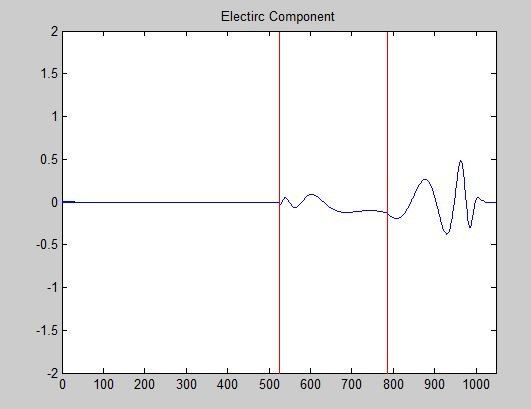
\includegraphics[width=5in]{Figures/drude3.jpg}
		%\rule{35em}{0.5pt}
	\caption[Gaussian Pulse after Passing through DNG slab]{conversion of Gaussian pulse into multiple wave forms of different frequencies after passing through dispersive DNG slab}
	\label{drude3}
\end{figure}

\begin{figure}[H]
	\centering
		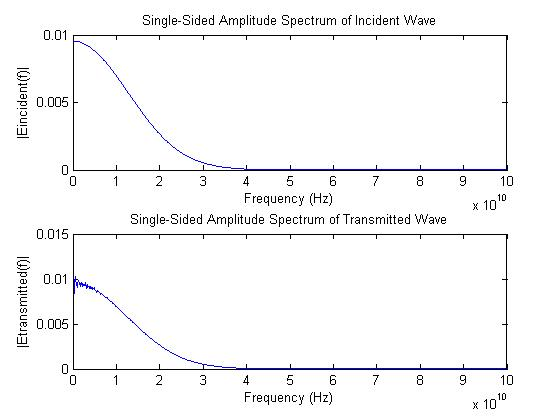
\includegraphics[width=5in]{Figures/drude5.jpg}
		%\rule{35em}{0.5pt}
	\caption[Reflected and Transmitted wave's Frequency Spectrum for 1D DNG simulation]{Reflected and Transmitted waves Frequency Spectrum for 1D DNG simulation with Gaussian wave as source}
	\label{drude5}
\end{figure}
\begin{figure}[H]
	\centering
		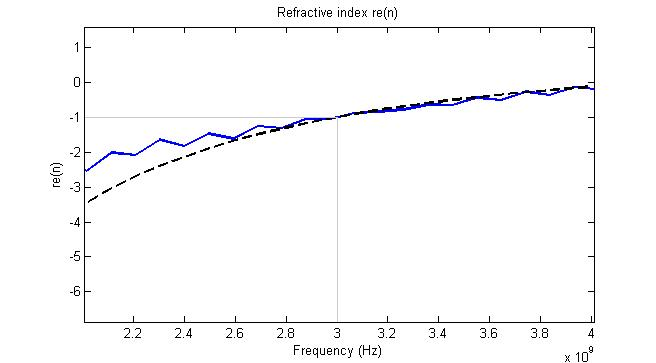
\includegraphics[width=5in]{Figures/drude4.jpg}
		%\rule{35em}{0.5pt}
	\caption[Refractive Index vs Frequency for 1D DNG slab]{Refractive indexes(Y-axis) Vs Frequency Graphs(X-axis) for 1D DNG slab, Black dashed line shows theoretical values, Blue line shows simulation results and calculated values, Grey lines mark the Frequency under study i.e 3GHz }
	\label{drude4}
\end{figure}
\textbf{Sinusoidal Source}\\
Figure \ref{drude2} shows the snapshot of simulation with Sinusoidal wave as source. it can be seen clearly that in steady state the wave entering the slab is identical to wave exiting the slab which implies that the reflected portion is approximately equal to zero. inside slab the wave seems to travel in opposite direction this is because the phase velocity\footnote{phase velocity of a wave is the rate at which the phase of the wave propagates in space} become negative inside NIM however the group velocity\footnote{group velocity of a wave is the velocity with which the overall shape of the waves' amplitudes ( known as the modulation or envelope of the wave) propagates through space.} is still in $-x$ direction.
\begin{figure}[H]
	\centering
		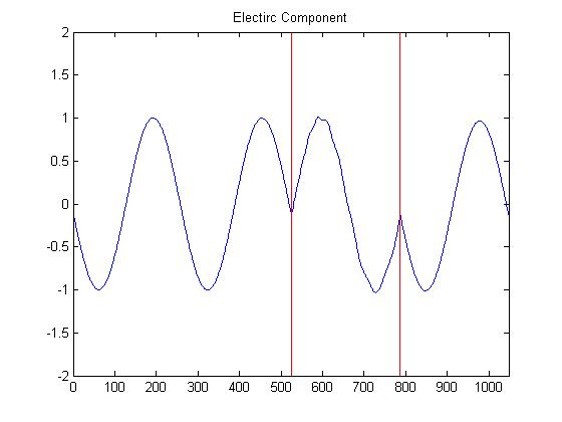
\includegraphics[width=5in]{Figures/drude2.jpg}
		%\rule{35em}{0.5pt}
	\caption[Sinusoidal wave passing through DNG slab]{Sinusoidal wave of 3Ghz passing through a slab of NIM}
	\label{drude2}
\end{figure}
%----------------------------------------------------------------------------------------
%	SECTION 3
%----------------------------------------------------------------------------------------

\section{Implementation in C++}
\index{C++ implementation}
Before implementing the code on GPU it needs to be converted in c++ as OpenCL use c99 which is similar to C.
). c++ have the basic functions to run the main loop, but it does not provide post processing utilities we require, natively, also graphical plotting is not supported. hence we must transfer the results of computation back to MATLAB for plotting and post processing.
%-----------------------------------
%	SUBSECTION 3.1
%-----------------------------------
\subsection{File handling in c++}
\index{File handling dynamic}
As our domain space can be very large the data produced by this computation is also very large. To transfer this data in MATLAB it have to be first written in files, but managing these files is also another issue. suppose we have a spatial domain of 2048, and time domain of 4084, it means there will be 2048 different values for each time step, as the simulation calculates both transmitted and refractive wave parameters total no of files become $2*Total_Time$ with each file having 2048 entries.
to cater this problem a dynamic file allocation scheme was written which saves the value for each time step in separate file and automatically name it accordingly.
\lstset{language=[ISO]C++, commentstyle=\color{green!50!black}, keywordstyle=\color{blue}, stringstyle=\color{red!60!black},caption=c++ file handling variables and Directory creation, label=cright1}
\begin{lstlisting}
// -------- Save to file Variables -------- 
	fstream snapshot;
	std::string filename ;
	std::stringstream stream;
	stream<<"results";
	CreateDirectory(stream.str().c_str(), NULL) ;		//create directory of results
\end{lstlisting}
this code \ref{cright1} creates a directory named results to store the files in current project directory. header file \emph{windows.h} is required for this command.
\lstset{language=[ISO]C++, commentstyle=\color{green!50!black}, keywordstyle=\color{blue}, stringstyle=\color{red!60!black},caption=c++ file handling using auto naming of file, label=cright2}
\begin{lstlisting}
// -------- Saving to file -------- 
	stream.str(std::string());   						// clear stringstream
	stream<<"./results/"<<"Efield"<<medium<<"_"<<qTime<<".jd";   		// concatenate
	filename = stream.str();		 					// copy string
	snapshot.open(filename, ios::out|ios::binary);
	for (mm = 0; mm < SIZE; mm++)
		snapshot.write((char *)&ez[mm],sizeof(double));
	snapshot.close();
\end{lstlisting}
Above code \ref{cright2} runs in the main time loop and saves values of Efield at every iteration. it automatically name the file according to medium and time instance. .jd is a file extension of own choice. Complete code can be found in Appendix \ref{cplus1}

Post processing and simulation movie is done by using MATLAB. below is the code to read the files written by c++ program
\lstset{language=Matlab, commentstyle=\color{green!50!black}, keywordstyle=\color{blue}, stringstyle=\color{red!60!black},caption=Read files in MATLAB, label=matread}
\begin{lstlisting}
	filepath=fullfile(pwd, 'results'); %set files directory path, pwd gets the current directory path
	% in main Time loop
	fidp = fopen(strcat(filepath,'\Efield',int2str(medium),'_',int2str(j),'.jd'),'r','l');
	        if fidp==-1
           	 display('Error');
       	        return
        	end
\end{lstlisting}
the code \ref{matread}  reads the files or else generate Error. $j$ is the variable used for main timing loop. with addition to these Efield values other simulation parameters are also written on individual files these parameters include Etransmitted, Ereflected, Ez1, Ez2 and simulation parameters (delta, k0, z1,z2). complete MATLAB code can be found in Appendix \ref{cplus2}
\clearpage
%----------------------------------- 
%	SECTION 4
%-----------------------------------
\section{Implementation on GPU }
\index{GPU}
Graphical Processing Unit or GPU is a computational device designed with a different architecture and different purpose. GPUs are Faster than CPUs because they have more number of cores (up-to 512 on a single chip \cite{cpuvsgpunotes}
) as compared to CPU and they use techniques like pipelining \cite{ref:gpu2}. GPUs memory is faster due to a larger bus width. simulations on GPU are 10-30 times faster than CPU \cite{Ref:gpuvscpui}
. Hence the FDTD algorithm is implemented on GPU because it can be parallelized.

%-----------------------------------
%	SUBSECTION 4.2
%-----------------------------------
\subsection{OpenCL}
\index{OpenCL}
OpenCL (Open Computing Language) is a framework by KHRONOS Group \cite{Khronos}
for parallel programming on heterogeneous systems. its main advantage is program portability, the same code can run on multiple devices such as CPU, GPU, FPGA, DSP kit \cite{ref:devices}
 etc. OpenCL framework include support for c++ however main kernels are written in language c99 which is a old standard for c language.
%-----------------------------------
%	SUBSECTION 4.3
%-----------------------------------
\subsection {OpenCL Program Flow}
To write a program in OpenCL we need to take care of Host side program, Kernel program, host side memory and device memory. the host is programmed in C/C++ while device is programmed using OpenCL C (c99).

\subsubsection{Kernel}
\index{Kernel function}
every function which runs on device is required to be in a kernel function

\lstset{language=C,caption=OpenCL Kernel function, label=kernel}
\begin{lstlisting}
__kernel void hy_kernel(__global PRECISION *hy, __global PRECISION *ez, __global PRECISION *mu, const PRECISION delt, const PRECISION delx, const int SIZE) 
{
	unsigned int i = get_global_id(0);
  if(i < SIZE)
    hy[i] = hy[i] + (ez[i+1] - ez[i]) * (delt/(delx*mu[i]));
}
\end{lstlisting}
OpenCl automatically manages \lstinline{global_id} and run them in parallel hence the multiplication result of  \lstinline{hy[i] = hy[i] + (ez[i+1] - ez[i]) * (delt/(delx*mu[i]));} are obtained simultaneously over the whole space.
\lstinline{__global PRECISION *hy} is used to pass an array into device memory. The kernel is only allowed read/write access to global, constant, local, and private memory, which is specified by \lstinline{ __global, __constant, __local, __private}, respectively. Kernel Functions can be found in \ref{gpu22}

\subsubsection{Host Program}
\label{HostProgram}
Host program executes the kernels using the API of OpenCL. Before running any program it initializes some parameters. In a complete run it performs a number of operations. which are listed below \cite{openclpro}.
\begin{enumerate}
\item Listing available platforms
\item Displaying platforms and get input for desired platform
\item Creating context
\item Creating command queue
\item Creating memory objects
\item Reading kernel file
\item Creation of program object
\item Compilation of kernel
\item Creating kernel object
\item Set kernel argument
\item Executing kernel
\item reading memory object
\item Releasing kernel
\item De-allocating memory in device
\end{enumerate}
\begin{figure}[H]
	\centering
		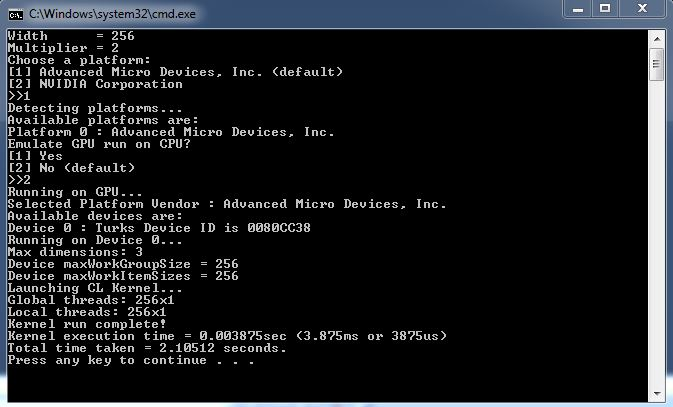
\includegraphics[width=6in]{Figures/opencl.jpg}
		%\rule{35em}{0.5pt}
	\caption[OpenCL basic run]{ Basics tasks performed by OpenCL API}
	\label{opencl}
\end{figure}

Complete codes can be found at \url{https://code.google.com/p/gpu-em-nim/source/browse/}
. After simulation post processing is done in MATLAB
%-----------------------------------
%	SUBSECTION 4.4
%-----------------------------------
\subsection {Challenges in GPU programming}
Main challenges in writing OpenCL program were

\subsubsection{Read Delay}
When data is passed to GPU or values are read from device memory to host memory considerable time is consumed. as in algorithm for boundary conditions we need previous time step values so there were a lot of data transfer from host to device and device to host memory, and to save the values of Electric field arrays they need to be brought into host memory. to reduce the overhead time absorbing boundary condition was moved into kernel number 2, and snapshot (writing to file) interval was changed from each iteration to every 20th iteration \ref{kernel2}.
\lstset{language=C,caption=OpenCL saving Efield values in files, label=kernel2}
\begin{lstlisting}
if (qTime % 20 ==0) // Snapshot interval
{
      //// Copy data back to host ////
      SafeCall(clEnqueueReadBuffer(commandQueue, ez_gpu, CL_TRUE, 0,  sizeof(PRECISION)*SIZE, ez, 0, NULL, NULL), "Error reading ez back to host memory");    
      SafeCall(clWaitForEvents(1, &events[0]), "Error: Waiting for kernel run to finish. (clWaitForEvents)");
         // -------- Saving to file -------- 
			stream.str(std::string());   						// clear stringstream
			stream<<"./results/"<<"Efield"<<medium<<"_"<<qTime+1<<".jd";   		// concatenate
			filename = stream.str();		 					// copy string
			snapshot.open(filename.c_str(), ios::out|ios::binary);
			for (mm = 0; mm < SIZE; mm++)
			snapshot.write((char *)&ez[mm],sizeof(float));
			snapshot.close();
 } 
\end{lstlisting}

\subsubsection{Kernel synchronization}
\index{Kernel synchronization}
As value of electric node depends on neighboring magnetic field nodes and value of magnetic field nodes  depends on neighboring electric field nodes it is essential that all kernels run in a synchronized way, or else wrong values would be calculated because of unavailability of updated nodes values. because all kernels are not performing same calculations it is prone to synchronization. to run these kernel in synchronized method following command \ref{kernel3}  is used inside kernel 2. this command basically look for global (other) kernel speed ad it's local speed, then it adds a delay to synchronize it perfectly with other kernels. there is a trade off with this method which is extra computational time in which the kernel is just waiting for others to complete.
\lstset{language=C,caption=Kernel synchronization, label=kernel3}
\begin{lstlisting}
	barrier(CLK_GLOBAL_MEM_FENCE|CLK_LOCAL_MEM_FENCE);
\end{lstlisting}











 
% Chapter Template

\chapter{Performance Analysis and Comparison} % Main chapter title

\label{Chapter3} % Change X to a consecutive number; for referencing this chapter elsewhere, use \ref{ChapterX}

\fancyhead[RO]{\thepage}
\fancyhead[RE]{\thepage}
\fancyhead[LE]{Chapter 3.~\emph{\Chaptername}}
\fancyhead[LO]{\emph{\ttitle}}

%----------------------------------------------------------------------------------------
%	SECTION 1
%----------------------------------------------------------------------------------------

\section{Computational time comparison}
same program was run on different platforms with same simulation parameters. These platforms were GPU, MATLAB (CPU), c++ (CPU) more details about these platforms can be found in Appendix B %ref here
Time domain is set to 1024,\\
Spatial domain values are $2^{10} - 2^{24}$,\\
Rest of the simulation parameters are enlisted in Appendix %ref here
\index{Performance comparison results, GPU C++ Matlab}
\begin{figure}[htbp]
	\centering
		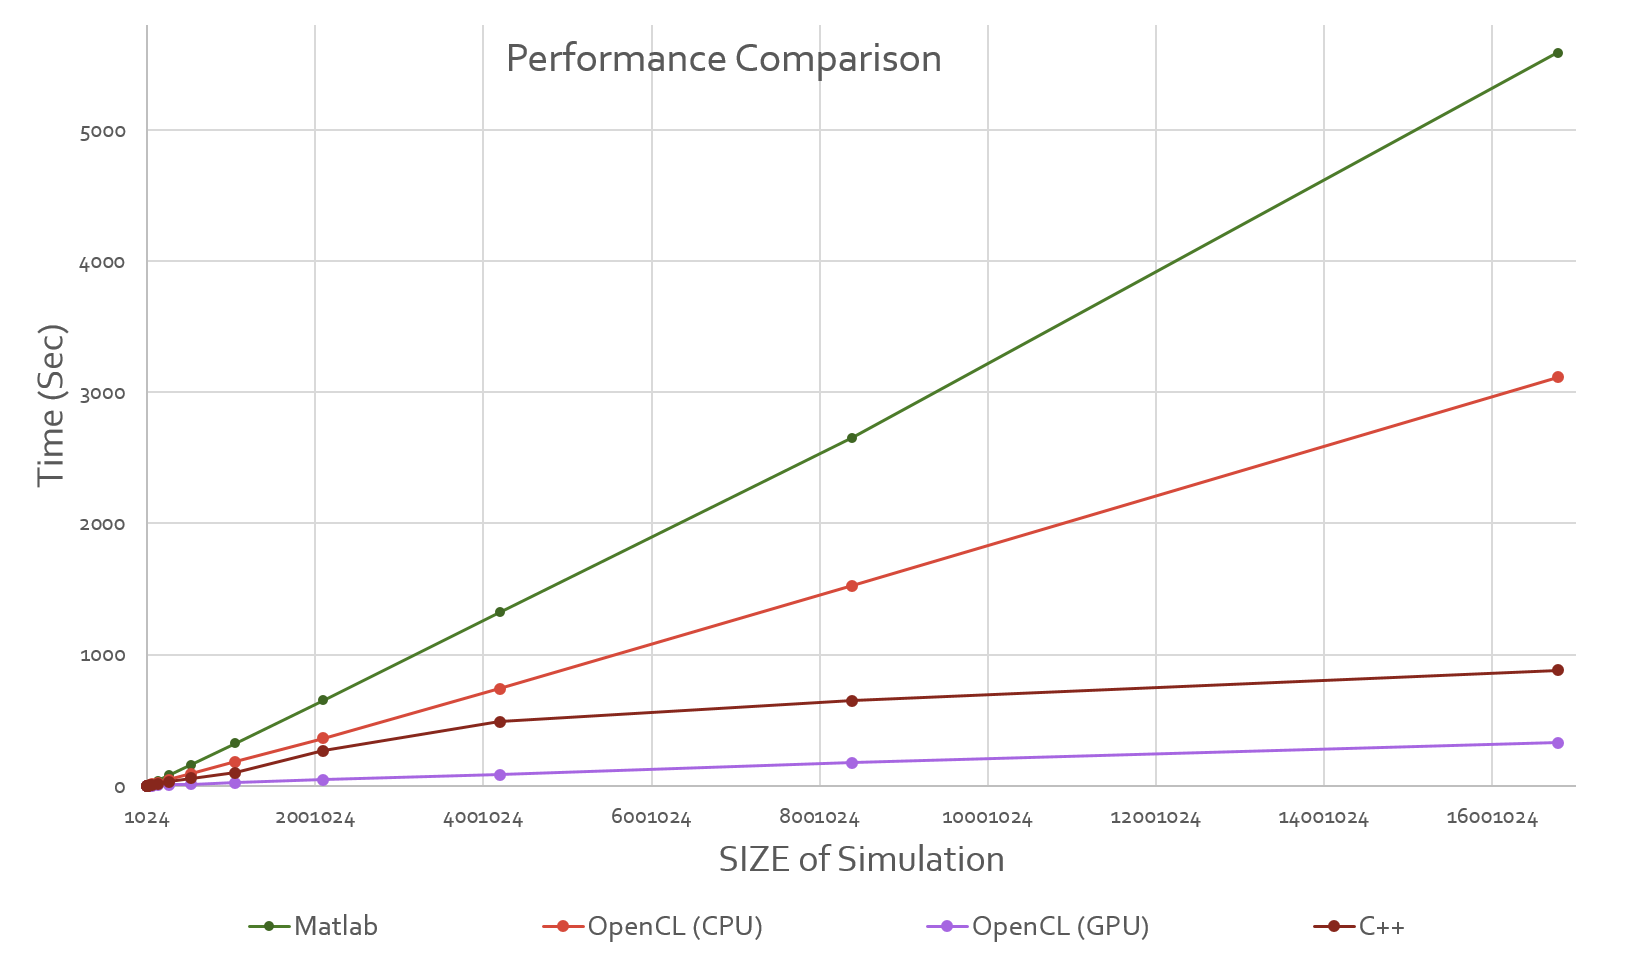
\includegraphics[width=6in]{Figures/g1.png}
	\caption[Computational Time on different platforms]{Performance comparison of computational time for different platforms over a large spatial domain $ Size = 2^{10} - 2^{24}$ }
	\label{g1}
\end{figure}
\begin{figure}[htbp]
	\centering
		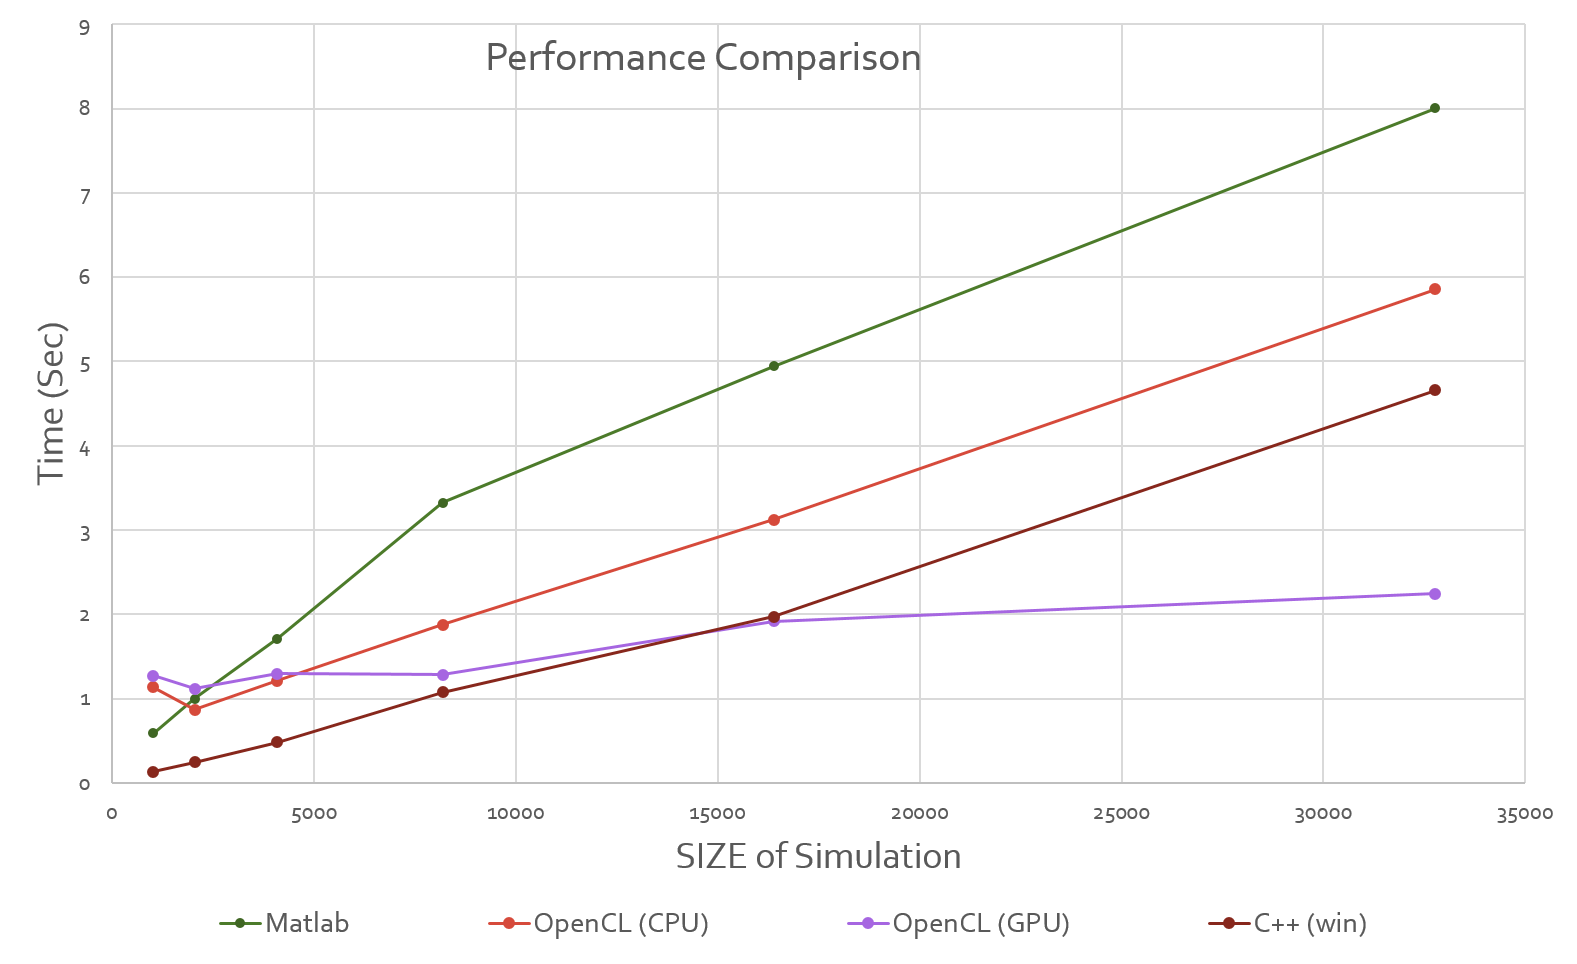
\includegraphics[width=6in]{Figures/g2.png}
	\caption[Computational Time on different platforms 2]{Performance comparison of computational time for different platforms for small size simulations $ Size = 2^{10} - 2^{15}$}
	\label{g2}
\end{figure}
\begin{figure}[htbp]
	\centering
		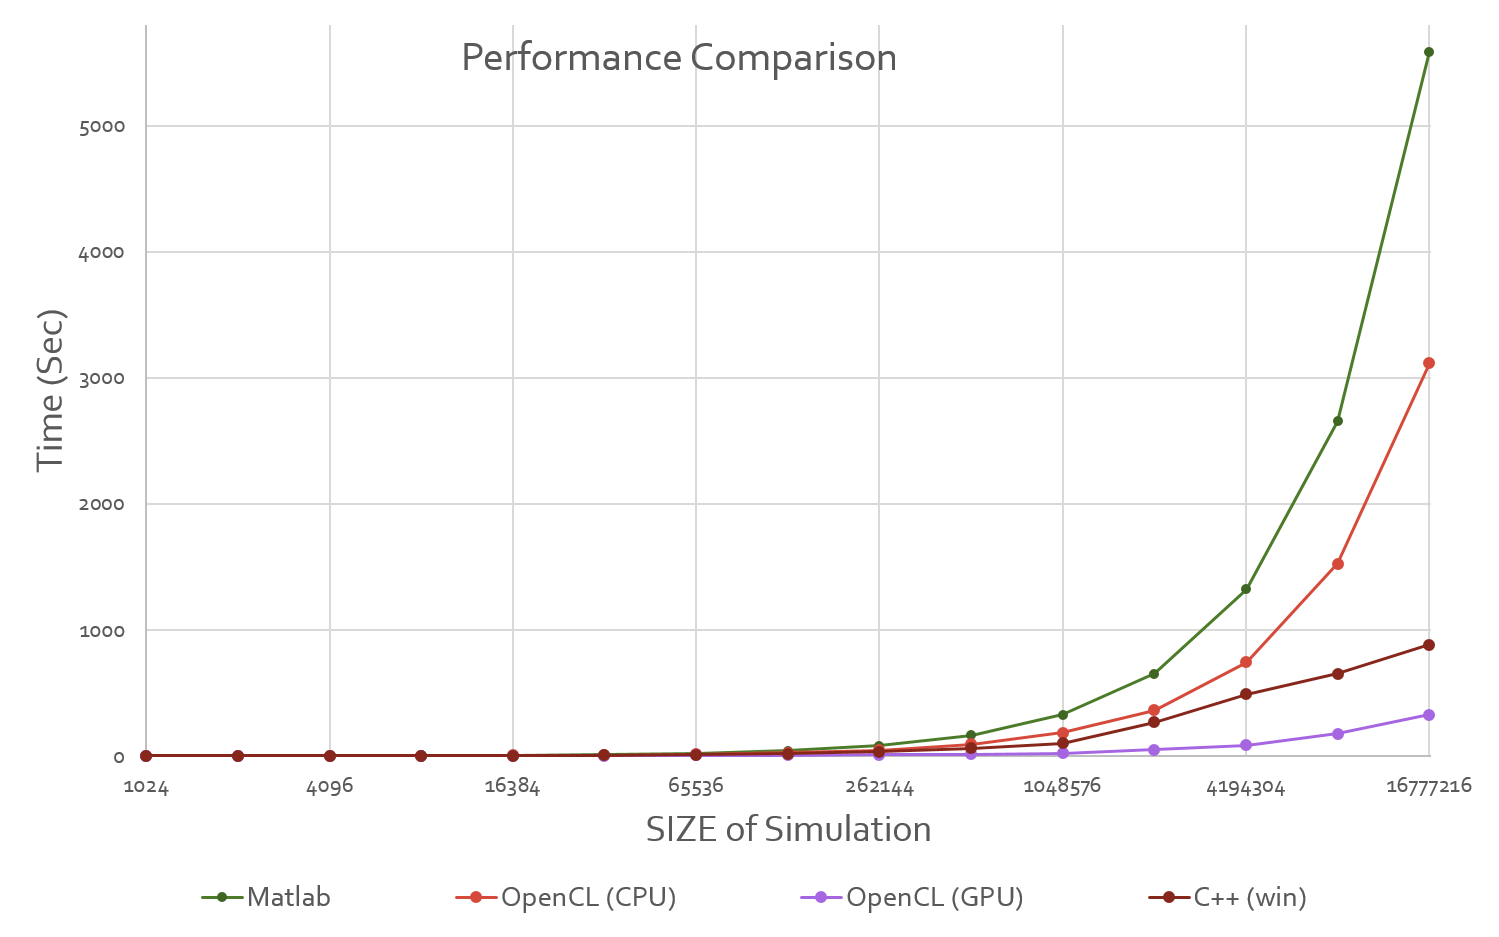
\includegraphics[width=6in]{Figures/g3.png}
	\caption[Performance Comparison on log scale]{Performance comparison of computational time for different platforms plotted over log scale}
	\label{g3}
\end{figure}

%-----------------------------------
%	SUBSECTION 2
%-----------------------------------
\section{Analysis }

From figure \ref{g1} it can be clearly observed that  computational time of GPU      is lowest and in term of few seconds even far larger domain size. it is 3 times better than that of C++ and           20 times better than MATLAB. These results can be improved by using a high end GPU or by using desktop version of GPU because in this case CPU (i7) is comparable to GPU (AMD 6770 Mobile).\\
Figure \ref{g2} shows the same results but it is plotted against on a relatively small domain size. here we can see the transitions in results. GPU is taking almost same time for lower simulation sizes this is because GPU takes some time to initialize  (see \nameref{HostProgram} on page \pageref{HostProgram}). the crossover point can be seen to be $2^{14}$.\\
Figure \ref{g3} shows the performance on a logarithmic $2^n$ x-axis, as we increase the domain size only in powers of two because of GPU kernels are in power of 2 and we do not want hardware resources to be underutilized. from this graph we can see the trend and also we can predict the computational time for each platform if we increase the domain size from $2^k  to  2^{k+1}$. 


%----------------------------------------------------------------------------------------
%	SECTION 2
%----------------------------------------------------------------------------------------

\section{Conclusion and Future Work}


%-----------------------------------
%	SUBSECTION 1
%-----------------------------------
\subsection{Conclusion }
FDTD algorithm was successfully implemented with Drudes model. All the parameters have been established and results are accurate when compared to theoretical values. Whole program was implemented on GPU and a significant reduction in computational time was achieved. it is observed that for small size simulations CPU gives a better performance than GPU, it also saves us from complex programming.


%-----------------------------------
%	SUBSECTION 2
%-----------------------------------
\subsection{Future Work }

There are number of applications of Negative index material, now that a basic platform is available and it is optimized for big simulations hence those applications can be modeled and researched further. Some interesting applications include Fiber optic design; for longer distances, RADAR absorbent; can be used in military applications as RAM, Photo-voltaic cell; with increased efficiency, Super lens; a lens with theoretical infinite zoom capabilities which can go beyond diffraction limits of conventional lens. the options are endless and with advancement of technology it is possible to not only research these fields but actually implement these modeled designs into physical designs. Negative index materials are a hot research topic in field of Electromagnetic field with a lot of known uses till date, it can be further explored for new uses and applications.


%% Chapter Template

\chapter{Experimental Results and Conclusion} % Main chapter title

\label{Chapter4} % Change X to a consecutive number; for referencing this chapter elsewhere, use \ref{ChapterX}

\lhead{Chapter 4. \emph{Results}} % Change X to a consecutive number; this is for the header on each page - perhaps a shortened title

%----------------------------------------------------------------------------------------
%	SECTION 1
%----------------------------------------------------------------------------------------

\section{Experimental Evalution}


%-----------------------------------
%	SUBSECTION 1
%-----------------------------------
\subsection{Frequency Response of Hydrophones }

There are a number of wireless communication techniques in underwater channel. These include acoustic, electromagnetic and optical mode. However, these techniques have problems which reduce the efficiency of communication in underwater channel. The reduced efficiency effects data rate, communication range and and Electromagnetic wave does not work well in underwater environment since because of its conduction most of the wave energy is absorbed by the channel.
Similarly optical mode is also not preferred due to scattering of light in underwater channel.
However acoustics is the most popular mode of underwater communication as it is least attenuated by the channel, which allows communication over long ranges. 
\begin{figure}[htbp]
	\centering
		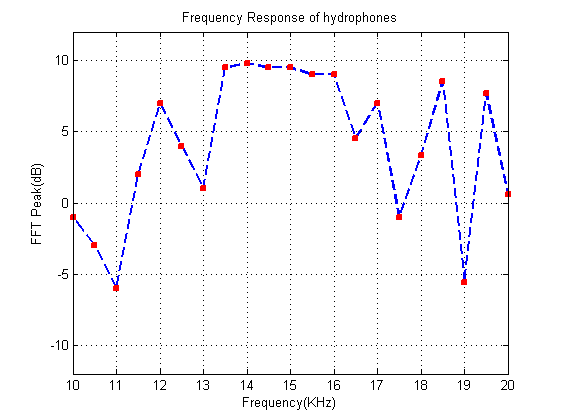
\includegraphics[width=5in]{Figures/Freq_response.png}
		\rule{35em}{0.5pt}
	\caption[Frequency Response of the Hydrophone]{Frequency Response of the Hydrophone.}
	\label{fig:freq}
\end{figure}

%-----------------------------------
%	SUBSECTION 2
%-----------------------------------
\subsection{Directivity Pattern of Hydrophones }

There are a number of wireless communication techniques in underwater channel. These include acoustic, electromagnetic and optical mode. However, these techniques have problems which reduce the efficiency of communication in underwater channel. The reduced efficiency effects data rate, communication range and and Electromagnetic wave does not work well in underwater environment since because of its conduction most of the wave energy is absorbed by the channel.
Similarly optical mode is also not preferred due to scattering of light in underwater channel.
However acoustics is the most popular mode of underwater communication as it is least attenuated by the channel, which allows communication over long ranges. 

%-----------------------------------
%	SUBSECTION 3
%-----------------------------------
\subsection{Transmission Range of Hydrophones }

There are a number of wireless communication techniques in underwater channel. These include acoustic, electromagnetic and optical mode. However, these techniques have problems which reduce the efficiency of communication in underwater channel. The reduced efficiency effects data rate, communication range and and Electromagnetic wave does not work well in underwater environment since because of its conduction most of the wave energy is absorbed by the channel.
Similarly optical mode is also not preferred due to scattering of light in underwater channel.
However acoustics is the most popular mode of underwater communication as it is least attenuated by the channel, which allows communication over long ranges. 
\begin{figure}[htbp]
	\centering
		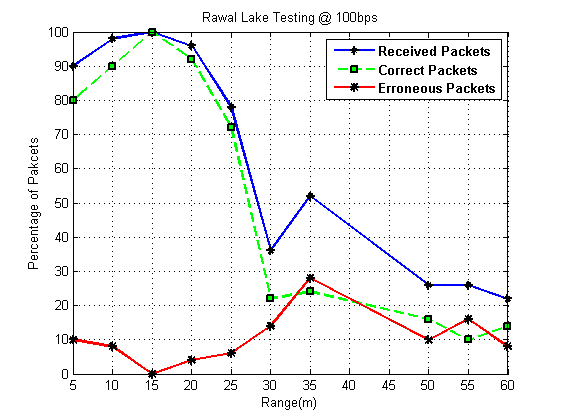
\includegraphics[width=5in]{Figures/Rawal_dam.png}
		\rule{35em}{0.5pt}
	\caption[Range Testing of the Hydrophones]{Range Testing of the Hydrophones.}
	\label{fig:rawal}
\end{figure}

%-----------------------------------
%	SUBSECTION 4
%-----------------------------------
\subsection{Evaluation of Testbed }

In this section we would evaluate the overall performance of our platform in terms of automation and communications so as to validate the claims made in previous sections.
1-	Evaluation Setup: the Platform evaluations setup is as show in the figure. We perform the experiments in specially designed pool measuring 20’ X 10’ in length and width respectively. For each physical point we send 500 packets and then evaluate the performance in terms of packet sent, received and lost. 
2-	Figure O shows the user interfaces(UI) for our web front. Figure Oa show the home page and Ob shows the experimentation page. You are required to fill in the details 

\begin{figure}[htbp]
	\centering
		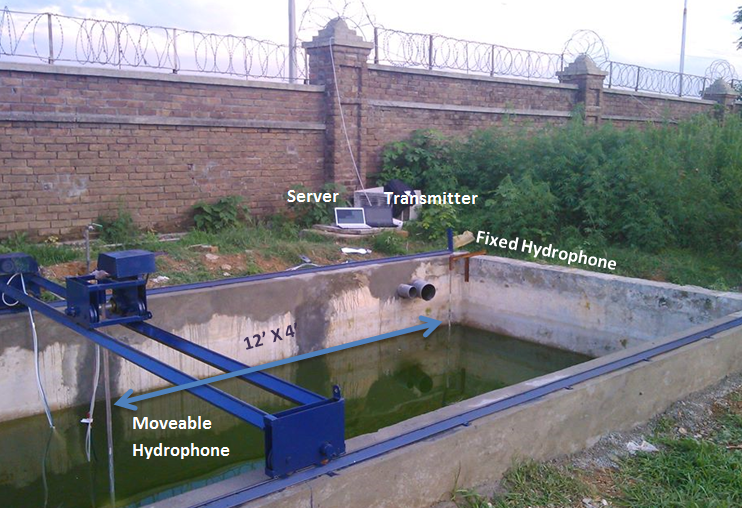
\includegraphics[width=5in]{Figures/setup11.png}
		\rule{35em}{0.5pt}
	\caption[Evaluation Setup of the Testbed]{Evaluation Setup of the Testbed.}
	\label{fig:evaluation}
\end{figure}


\begin{figure}[htbp]
	\centering
		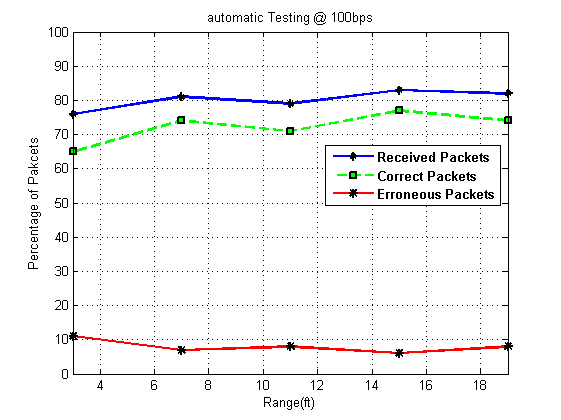
\includegraphics[width=5in]{Figures/results.png}
		\rule{35em}{0.5pt}
	\caption[Evaluation Result of the Testbed]{Evaluation Result of the Testbed.}
	\label{fig:evaluation_results}
\end{figure}


%----------------------------------------------------------------------------------------
%	SECTION 2
%----------------------------------------------------------------------------------------

\section{Conclusion and Future Work}


%-----------------------------------
%	SUBSECTION 1
%-----------------------------------
\subsection{Conclusion }

There are a number of wireless communication techniques in underwater channel. These include acoustic, electromagnetic and optical mode. However, these techniques have problems which reduce the efficiency of communication in underwater channel. The reduced efficiency effects data rate, communication range and and Electromagnetic wave does not work well in underwater environment since because of its conduction most of the wave energy is absorbed by the channel.
Similarly optical mode is also not preferred due to scattering of light in underwater channel.
However acoustics is the most popular mode of underwater communication as it is least attenuated by the channel, which allows communication over long ranges. 

%-----------------------------------
%	SUBSECTION 2
%-----------------------------------
\subsection{Future Work }

There are a number of wireless communication techniques in underwater channel. These include acoustic, electromagnetic and optical mode. However, these techniques have problems which reduce the efficiency of communication in underwater channel. The reduced efficiency effects data rate, communication range and and Electromagnetic wave does not work well in underwater environment since because of its conduction most of the wave energy is absorbed by the channel.
Similarly optical mode is also not preferred due to scattering of light in underwater channel.
However acoustics is the most popular mode of underwater communication as it is least attenuated by the channel, which allows communication over long ranges. 

 
%\input{Chapters/Chapter5} 
%\input{Chapters/Chapter6} 
%\input{Chapters/Chapter7} 

%----------------------------------------------------------------------------------------
%	THESIS CONTENT - APPENDICES
%----------------------------------------------------------------------------------------

\addtocontents{toc}{\vspace{2em}} % Add a gap in the Contents, for aesthetics

\appendix % Cue to tell LaTeX that the following 'chapters' are Appendices

% Include the appendices of the thesis as separate files from the Appendices folder
% Uncomment the lines as you write the Appendices

% Appendix A

\chapter{Program codes} % Main appendix title

\label{AppendixA} % For referencing this appendix elsewhere, use \ref{AppendixA}

\lhead{Appendix A. \emph{Program codes}} % This is for the header on each page - perhaps a shortened title

%-------------------------------------------------------------------
\textbf{SVN Link:} \url{https://code.google.com/p/gpu-em-nim/}

\lstset{language=Matlab, commentstyle=\color{green!50!black}, keywordstyle=\color{blue}, stringstyle=\color{red!60!black},caption=FDTD Free space simulation,label=matlab1}
\begin{lstlisting}
SIZE=201;
ez=zeros(1,SIZE);
hy=zeros(1,SIZE);
imp0=377; %squareroot(u0/e0)
maxTime = 1001;
mm=0;
temp=0;
    for qTime = 1:(maxTime-1)
%        Update Magnetic field
        for  mm = 1:(SIZE - 2)
            hy(mm) = hy(mm) + (ez(mm + 1) - ez(mm)) / imp0;
        end
%         Update Electrical filed
        for mm = 2:(SIZE-1)
            ez(mm) = ez(mm) + (hy(mm) - hy(mm - 1)) * imp0;
        end
%         Source node (hard coded)
        ez(1) = exp(-(qTime - 30) * (qTime - 30) / 100.);
%         Plotting
        figure(1);
        grid on; 
        subplot(2,1,1);
        plot(1:SIZE,ez);
        title('Electirc Component');
        Xlim([0 SIZE]);
        ylim([-1.2 1.2]);
        subplot(2,1,2);
        plot(1:SIZE,hy);
        title('Magnetic Component');
        Xlim([0 SIZE]);
        ylim([-0.003 0.003]);
        pause(0.02);
    end
	
\end{lstlisting}

\lstset{language=Matlab, commentstyle=\color{green!50!black}, keywordstyle=\color{blue}, stringstyle=\color{red!60!black},caption=Perfect magnetic conductor boundary condition,label=matlab2}
\begin{lstlisting}
SIZE=201;
ez=zeros(1,SIZE);
hy=zeros(1,SIZE);
mu=[1.2566e-006*ones(1,SIZE)];   %permeability of free sapce
% epsilon=[8.8542e-012*ones(1,SIZE)]; %permittivity of free space 
epsilon=[8.8542e-012*ones(1,SIZE-80) 1.7708e-011*ones(1,20) 8.8542e-012*ones(1,60)]; %introducing medium of 2*e with a width of 20
% ideal Condition --> Sc= c*delt/delx = 1
delt=1;
delx=299792458;
maxTime = 1001;
mm=0;
temp=0;
    for qTime = 1:(maxTime-1)
%        Update Magnetic field
        for  mm = 1:(SIZE - 2)
            hy(mm) = hy(mm) + (ez(mm + 1) - ez(mm)) * (delt/(delx*mu(mm)));
        end
%         Update Electrical filed
        for mm = 2:(SIZE-1)
            ez(mm) = ez(mm) + (hy(mm) - hy(mm - 1)) * (delt/(delx*epsilon(mm))) ;
        end
%         Source node (hard coded)
        ez(1) = exp(-(qTime - 30) * (qTime - 30) / 100.);
%         Plotting
        figure(1);
        grid on; 
        subplot(2,1,1);
        plot(1:SIZE,ez);
        title('Electirc Component');
        Xlim([0 SIZE]);
        ylim([-1.5 1.5]);
        line([SIZE-80 SIZE-80],[-1.5 1.5],'Color','Red')
        line([SIZE-60 SIZE-60],[-1.5 1.5],'Color','Red')
        subplot(2,1,2);
        plot(1:SIZE,hy);
        title('Magnetic Component');
        Xlim([0 SIZE]);
        ylim([-0.005 0.005]);
        line([SIZE-80 SIZE-80],[-0.005 0.005],'Color','Red')
        line([SIZE-60 SIZE-60],[-0.005 0.005],'Color','Red')
        pause(0.02);
    end
\end{lstlisting}

\lstset{language=Matlab, commentstyle=\color{green!50!black}, keywordstyle=\color{blue}, stringstyle=\color{red!60!black},caption=Absorbing boundary condition (ABC),label=matlab3}
\begin{lstlisting}
clc;
SIZE=201;
ez=zeros(1,SIZE);
hy=zeros(1,SIZE-1);

% Medium Specifications
mu=[1.2566e-006*ones(1,SIZE)];   %permeability of free sapce
% epsilon=[8.8542e-012*ones(1,SIZE)]; %permittivity of free space 
epsilon=[8.8542e-012*ones(1,SIZE-80) 1.7708e-011*ones(1,20) 8.8542e-012*ones(1,60)]; %introducing medium of 2*e with a width of 20

% Courant Number (Accuracy) Sc
% ideal Condition --> Sc= c*delt/delx = 1
delt=1;
delx=299792458;
Sc=299792458*delt/delx;
epsilonr=1;
mur=1;

maxTime = 1001;
mm=0;
temp=0;
ez1q=0;
ez2q=0;
ezmq=0;
ezm1q=0;
    for qTime = 1:(maxTime-1)
%        Update Magnetic field
        for  mm = 1:(SIZE-1)
            hy(mm) = hy(mm) + (ez(mm + 1) - ez(mm)) * (delt/(delx*mu(mm)));
        end
%         Update Electrical filed
        for mm = 2:(SIZE-1)
            ez(mm) = ez(mm) + (hy(mm) - hy(mm - 1)) * (delt/(delx*epsilon(mm))) ;
        end
%         Source node (hard coded)
        ez(2) = ez(2)+exp(-(qTime - 30) * (qTime - 30) / 100.); %additive Source
%         Absorbing Boundary Conditions
        ez(1)=ez2q+(ez(2)-ez1q)*(((Sc/(mur*(epsilonr))^0.5)-1)/((Sc/(mur*(epsilonr))^0.5)+1));
        ez(SIZE)=ezm1q+(ez(SIZE-1)-ezmq)*(((Sc/(mur*(epsilonr))^0.5)-1)/((Sc/(mur*(epsilonr))^0.5)+1));
%         Saving q-1 (pervious step time values) for boundary Conditions
        ez2q=ez(2);
        ez1q=ez(1);
        ezmq=ez(SIZE);
        ezm1q=ez(SIZE-1);
%         Plotting
        figure(1);
        grid on; 
        subplot(2,1,1);
        plot(1:SIZE,ez);
        title('Electirc Component');
        xlim([0 SIZE]);
        ylim([-1.2 1.2]);
        line([SIZE-80 SIZE-80],[-1.2 1.2],'Color','Red') % Medium slab line
        line([SIZE-60 SIZE-60],[-1.2 1.2],'Color','Red') % Medium slab line
        subplot(2,1,2);
        plot(1:SIZE-1,hy);
        title('Magnetic Component');
        xlim([0 SIZE]);
        ylim([-0.005 0.005]);
        line([SIZE-80 SIZE-80],[-0.005 0.005],'Color','Red') % Medium slab line
        line([SIZE-60 SIZE-60],[-0.005 0.005],'Color','Red') % Medium slab line
        pause(0.02);
    end
\end{lstlisting}

\lstset{language=Matlab, commentstyle=\color{green!50!black}, keywordstyle=\color{blue}, stringstyle=\color{red!60!black},caption=Complete 1D FDTD implementation wiht Post Processing,label=matlab4}
\begin{lstlisting}
clc;
SIZE=1024;   
maxTime =1024;

SourceSelect=1; % 0=Sinosoidal, 1=Gauassian

%Constants
c=3e8;

% Courant Number (Accuracy) Sc
% ideal Condition --> Sc= c*delt/delx = 1
% f=3Ghz, lambda=c/f=0.1m, for 4 wavelengths, dx=0.4/(maxtime=1000)
PulseWidth=800;
f=3e9;
w=2*pi*f;    % omega
k0=w/c     ; % free space wave number constant
lambda=c/f;
delx=(4*lambda)/SIZE;
% so dt=dx/c=1.333e-12
delt=delx/c;
Sc=c*delt/delx;
epsilonr=1;
mur=1;


% Incident and Refelected Waves Variables
Eincident=0;
Etransmitted=0;
Etemp=zeros(1,maxTime);


% refractive index variables
Z1 = 750;
z1 = Z1*delx;
Z2 = 760;
z2 = Z2*delx;
Exz1 = zeros(maxTime,1); % record Electric field at 750
Exz2 = zeros(maxTime,1); % record electric field at 760
fspan = 100; % Points to plot in frequency domain

for medium= 1:2
    % Temp Variable
    ez=zeros(1,SIZE);
    hy=zeros(1,SIZE-1);
    mm=0;
    ez1q=0;
    ez2q=0;
    ezmq=0;
    ezm1q=0;
    % Medium Specifications
    mu=1.2566e-006*ones(1,SIZE);   %permeability of free sapce
    if medium==1
        epsilon=8.8542e-012*ones(1,SIZE); % free space
    else
        epsilon=[8.8542e-012*ones(1,SIZE-500) 1.7708e-011*ones(1,500)]; % half medium
    end
    for qTime = 1:(maxTime-1)
%        Update Magnetic field
    	for  mm = 1:(SIZE-1)
            hy(mm) = hy(mm) + (ez(mm + 1) - ez(mm)) * (delt/(delx*mu(mm)));
        end
%         Update Electrical filed
        for mm = 2:(SIZE-1)
            ez(mm) = ez(mm) + (hy(mm) - hy(mm - 1)) * (delt/(delx*epsilon(mm))) ;
        end
        Etemp(qTime)= ez(SIZE-498); %just after boundary of medium
        if SourceSelect==0
%         Source node (hard coded)
		    ez(2) = ez(2)+ (sin(2*pi*(qTime)*f*delt)*Sc);
		else
		    ez(2) = ez(2)+exp(-(qTime - 30) * (qTime - 30) / (PulseWidth./4));
		end
%         Absorbing Boundary Conditions
        ez(1)=ez2q+(ez(2)-ez1q)*(((Sc/(mur*(epsilonr))^0.5)-1)/((Sc/(mur*(epsilonr))^0.5)+1));
        ez(SIZE)=ezm1q+(ez(SIZE-1)-ezmq)*(((Sc/(mur*(epsilonr))^0.5)-1)/((Sc/(mur*(epsilonr))^0.5)+1));
%         Saving q-1 (pervious step time values) for boundary Conditions
		ez2q=ez(2);
		ez1q=ez(1);
		ezmq=ez(SIZE);
		ezm1q=ez(SIZE-1);
%         Plotting
       if medium==2
         if mod(qTime,5)==0   
        figure(1);
        subplot(2,1,1);
        plot(1:SIZE,ez);
        title('Electirc Component');
        xlim([0 SIZE]);
        ylim([-1.2 1.2]);
        if medium==2
            line([SIZE-500 SIZE-500],[-1.2 1.2],'Color','Red') % Medium slab line
        end
        subplot(2,1,2);
        plot(1:SIZE-1,hy);
        title('Magnetic Component');
        xlim([0 SIZE]);
        ylim([-0.005 0.005]);
        if medium==2
        line([SIZE-500 SIZE-500],[-0.005 0.005],'Color','Red') % Medium slab line
        end
         end
       end
          Exz1(qTime)=ez(Z1);
          Exz2(qTime)=ez(Z2);
    end
    if medium==1
        Eincident=Etemp;
    else
        Etransmitted=Etemp;
    end
end
% Frequency Domain Analysis
Fs=1/delt;   %Sampling Frequency
T=1/Fs;      %Sample Time
L=maxTime;      %Length of Signal
time=(0:L-1)*T;    %Time Vector
figure(2);
subplot(2,1,1);
plot(Fs*time,Eincident)
title('Incident Wave');
xlabel('time (picoseconds)')
subplot(2,1,2);
plot(Fs*time,Etransmitted);
title('Transmitted Wave');
xlabel('time (picoseconds)')
% Fourrier Domain
NFFT = 2^nextpow2(L); % Next power of 2 from length of y
FEincident = fft(Eincident,NFFT)/L;
FEtransmitted = fft(Etransmitted,NFFT)/L;
f = Fs/2*linspace(0,1,NFFT/2+1);          %frequency scaling
% Plot single-sided amplitude spectrum.
figure(3);
subplot(2,1,1);
plot(f,2*abs(FEincident(1:NFFT/2+1))) 
xlim([0 1e11]);
% ylim([0 0.5]);
title('Single-Sided Amplitude Spectrum of Incident Wave')
xlabel('Frequency (Hz)')
ylabel('|Eincident(f)|')
subplot(2,1,2);
plot(f,2*abs(FEtransmitted(1:NFFT/2+1)))
xlim([0 1e11]);
% ylim([0 0.5]);
title('Single-Sided Amplitude Spectrum of Transmitted Wave')
xlabel('Frequency (Hz)')
ylabel('|Etransmitted(f)|')

cTransmitted=FEtransmitted/FEincident
cReflected=1-cTransmitted
eta1=sqrt(1/1);
eta2=sqrt(2/1);
Gamma=(eta2-eta1)/(eta2+eta1)


% eq 33
EXZ1 = fft(Exz1,NFFT)/L;
EXZ2 = fft(Exz2,NFFT)/L;

nFDTD = (1/(1i*k0*(z1-z2))).*log(EXZ2(1:NFFT/2+1)./EXZ1(1:NFFT/2+1));
figure(4);
plot(f(1:fspan), real(nFDTD(1:fspan)));
title('Refractive index re(n)');
xlabel('Frequency (Hz)');
ylabel('re(n)');
line([3e9 3e9],[-15 1.415],'Color','Red')
line([0e9 3e9],[1.415 1.415],'Color','Red')

ReferectiveIndex=(1/(k0*(760-750)*i))*log(FEtransmitted(760)/FEtransmitted(750))

\end{lstlisting}

\lstset{language=Matlab, commentstyle=\color{green!50!black}, keywordstyle=\color{blue}, stringstyle=\color{red!60!black},caption=Drudes Model,label=matlab5}
\begin{lstlisting}

%% Variables Section
clear;
clc;
snapshot=10;
SIZE=1048;   
maxTime =5*SIZE;

SourceSelect=1; % 0=Sinosoidal, 1=Gauassian

%Constants
c=3e8;

% Courant Number (Accuracy) Sc
% ideal Condition --> Sc= c*delt/delx = 1
PulseWidth=800;
f=3e9;      % 3GHz
w=2*pi*f;    % omega
k0=w/c     ; % free space wave number constant
lambda=c/f;
delx=(4*lambda)/SIZE;
% so dt=dx/c=1.333e-12
delt=delx/c;
Sc=c*delt/delx;
epsilonr=-1;
mur=-1;
mu_nought=1.2566e-006;
epsilon_nought=8.8542e-012;
% Drudes model variables
mu_inf=1;
    epsilon_inf=1;
    omega_pe2= 4*pi*pi*f*f*(epsilon_inf-epsilonr);%Plasma frequency electric squared
    omega_pm2= 4*pi*pi*f*f*(mu_inf-mur);%Plasma frequency magnetic squared
    ro_m=0;
    ro_e=0;
% Incident and Refelected Waves Variables
Eincident=0;
Etransmitted=0;
Etemp=zeros(1,maxTime);

% refractive index variables
Z1 = (SIZE/2)+100;
z1 = Z1*delx;
Z2 = (SIZE/2)+110;
z2 = Z2*delx;
Exz1 = zeros(maxTime,1); % record Electric field at 750
Exz2 = zeros(maxTime,1); % record electric field at 760
fspan = 100; % Points to plot in frequency domain
%% Main Loop
for medium= 1:2
    % Medium Specifications
    if medium==1
        mu=1.2566e-006*ones(1,SIZE);   %permeability of free sapce
        epsilon=8.8542e-012*ones(1,SIZE); % free space
        epsilonr=ones(1,SIZE);
        mur=ones(1,SIZE);
    else
        epsilon=[8.8542e-012*ones(1,SIZE-(SIZE/2)) -8.8542e-012*ones(1,(SIZE/4)) 8.8542e-012*ones(1,(SIZE/4))]; % half medium
        mu=[1.2566e-006*ones(1,SIZE-(SIZE/2)) -1.2566e-006*ones(1,(SIZE/4)) 1.2566e-006*ones(1,(SIZE/4))];
        epsilonr=[ones(1,SIZE-(SIZE/2)) -1*ones(1,SIZE/4) ones(1,SIZE/4)];
        mur=[ones(1,SIZE-(SIZE/2)) -1*ones(1,SIZE/4) ones(1,SIZE/4)];
    end
    for  mm = 1:(SIZE)
        omega_pe2= 4*pi*pi*f*f*(epsilon_inf-epsilonr(mm));%Plasma frequency electric squared
        omega_pm2= 4*pi*pi*f*f*(mu_inf-mur(mm));%Plasma frequency magnetic squared
        m_divide=((4*mu_nought*mu_inf)+(mu_nought*omega_pm2*(delt*delt))+(mu_nought*mu_inf*ro_m*(2*delt)));
        am(mm)= 4/m_divide;
        bm(mm)= (ro_m*2*delt)/m_divide;
        cm(mm)= (4*mu_nought*mu_inf)/m_divide;
        dm(mm)= (-mu_nought*omega_pm2*delt*delt)/m_divide;
        em(mm)= (mu_nought*mu_inf*ro_m*2*delt)/m_divide;
        e_divide=((4*epsilon_nought*epsilon_inf)+(epsilon_nought*omega_pe2*(delt*delt))+(epsilon_nought*epsilon_inf*ro_e*(2*delt)));
        ae(mm)= 4/e_divide;
        be(mm)= (ro_e*2*delt)/e_divide;
        ce(mm)= (4*epsilon_nought*epsilon_inf)/e_divide;
        de(mm)= (-epsilon_nought*omega_pe2*delt*delt)/e_divide;
        ee(mm)= (epsilon_nought*epsilon_inf*ro_e*2*delt)/e_divide;
    end
    % Temp Variable
    ez=zeros(1,SIZE);
    ezn_0=zeros(1,SIZE-1);
    ezn_1=zeros(1,SIZE-1);
    hy=zeros(1,SIZE-1);
    hyn_0=zeros(1,SIZE-1);
    hyn_1=zeros(1,SIZE-1);
    by=zeros(1,SIZE);
    byn_0=zeros(1,SIZE);
    byn_1=zeros(1,SIZE);
    dz=zeros(1,SIZE);
    dzn_0=zeros(1,SIZE);
    dzn_1=zeros(1,SIZE);
    mm=0;
    ez1q=0;
    ez2q=0;
    ezmq=0;
    ezm1q=0;
    
    for qTime = 1:(maxTime-1)
        % Drudes model Calculations
        %storing pervious time steps values
        hyn_1=hyn_0;
        hyn_0=hy;
        byn_1=byn_0;
        byn_0=by;
        ezn_1=ezn_0;
        ezn_0=ez;
        dzn_1=dzn_0;
        dzn_0=dz;
%        Update By
        for  mm = 1:(SIZE-1)
            by(mm) = by(mm) + ((ez(mm) - ez(mm+1)) * (delt/(delx)));
        end
%        Update Magnetic field
        for  mm = 1:(SIZE-1)  %changed it from 1 to 2 because of by(0) index problem at 1
            hy(mm) = (am(mm)*(by(mm)-2*byn_0(mm)+byn_1(mm)))+(bm(mm)*(by(mm)-byn_1(mm)))+(cm(mm)*((2*hyn_0(mm))-(hyn_1(mm))))+(dm(mm)*((2*hyn_0(mm))+(hyn_1(mm))))+(em(mm)*(hyn_1(mm)));
        end
%         Update Dz
        for mm = 2:(SIZE-1)
            dz(mm) = dz(mm) + ((hy(mm-1) - hy(mm)) * (delt/delx));
        end
%         Update Electrical filed
        for mm = 2:(SIZE-1)
            ez(mm) = (ae(mm)*(dz(mm)-(2*dzn_0(mm))+dzn_1(mm)))+(be(mm)*(dz(mm)-dzn_1(mm)))+(ce(mm)*((2*ezn_0(mm))-ezn_1(mm)))+(de(mm)*((2*ezn_0(mm))+ezn_1(mm)))+(ee(mm)*ezn_1(mm));
        end
        Etemp(qTime)= ez(SIZE-(SIZE/2)+2); %just after boundary of medium
        if SourceSelect==0
%         Source node (hard coded)
            ez(1) = (sin(2*pi*(qTime)*f*delt)*Sc);
            dz(1)=epsilonr(1)*epsilon_nought*ez(1);
         else
            ez(1)= exp(-(qTime - 30) * (qTime - 30) / (PulseWidth./4));
            dz(1)=epsilonr(1)*epsilon_nought*ez(1);
        end
%         Absorbing Boundary Conditions
        ez(SIZE)=ezm1q+(ez(SIZE-1)-ezmq)*(((Sc/(mur(1)*(epsilonr(1)))^0.5)-1)/((Sc/(mur(1)*(epsilonr(1)))^0.5)+1));
        dz(SIZE)=epsilonr(1)*epsilon_nought; 
%         Saving q-1 (pervious step time values) for boundary Conditions
		ez2q=ez(2);
		ez1q=ez(1);
		ezmq=ez(SIZE);
		ezm1q=ez(SIZE-1);
%         Plotting
       if medium==2
       if mod(qTime,snapshot)==0
        figure(1);
%         subplot(2,1,1);
        plot(1:SIZE,ez);
        title('Electirc Component');
        xlim([0 SIZE]);
%         ylim([-1.2 1.2]);
%         if medium==2
            line([SIZE-(SIZE/2) SIZE-(SIZE/2)],[-2 2],'Color','Red') % Medium slab line
            line([SIZE-(SIZE/4) SIZE-(SIZE/4)],[-2 2],'Color','Red') % Medium slab line
%         end
       end
       end
          Exz1(qTime)=ez(Z1);
          Exz2(qTime)=ez(Z2);
    end
    if medium==1
        Eincident=Etemp;
    else
        Etransmitted=Etemp;
    end
end
%% Post processing
% Frequency Domain Analysis
Fs=1/delt;   %Sampling Frequency
T=1/Fs;      %Sample Time
L=maxTime;      %Length of Signal
time=(0:L-1)*T;    %Time Vector
figure(2);
subplot(2,1,1);
plot(Fs*time,Eincident)
title('Incident Wave');
xlabel('time (picoseconds)')
subplot(2,1,2);
plot(Fs*time,Etransmitted);
title('Transmitted Wave');
xlabel('time (picoseconds)')
% Fourrier Domain
NFFT = 2^nextpow2(L); % Next power of 2 from length of y
FEincident = fft(Eincident,NFFT)/L;
FEtransmitted = fft(Etransmitted,NFFT)/L;
f = Fs/2*linspace(0,1,NFFT/2+1);          %frequency scaling
% Plot single-sided amplitude spectrum.
figure(3);
subplot(2,1,1);
plot(f,2*abs(FEincident(1:NFFT/2+1))) 
xlim([0 1e11]);
% ylim([0 0.5]);
title('Single-Sided Amplitude Spectrum of Incident Wave')
xlabel('Frequency (Hz)')
ylabel('|Eincident(f)|')
subplot(2,1,2);
plot(f,2*abs(FEtransmitted(1:NFFT/2+1)))
xlim([0 1e11]);
% ylim([0 0.5]);
title('Single-Sided Amplitude Spectrum of Transmitted Wave')
xlabel('Frequency (Hz)')
ylabel('|Etransmitted(f)|')

cTransmitted=FEtransmitted/FEincident
cReflected=1-cTransmitted
eta1=sqrt(1/1);
eta2=sqrt(-1/1);
Gamma=(eta2-eta1)/(eta2+eta1)


% eq 33
EXZ1 = fft(Exz1,NFFT)/L;
EXZ2 = fft(Exz2,NFFT)/L;

nFDTD = (1/(1i*k0*(z1-z2))).*log(EXZ2(1:NFFT/2+1)./EXZ1(1:NFFT/2+1));
figure(4);
%plot(f(1:fspan), real(nFDTD(1:fspan)));
plot(f(20:50), real(nFDTD(20:50)));
title('Refractive index re(n)');
xlabel('Frequency (Hz)');
ylabel('re(n)');
line([3e9 3e9],[-4 -1],'Color','Red')
line([1e9 3e9],[-1 -1],'Color','Red')

ReferectiveIndex=(1/(k0*(Z2-Z1)*i))*log(FEtransmitted(Z2)/FEtransmitted(Z1))

f0=3e9;
w0=2*pi*f0;
einf=1;
wpe2= 2*(w0^2);
f = 2e9:1e8:4e9;
length(f)

er = einf - wpe2./(2*pi*f).^2;
figure(4)
hold on
plot(f,er)
line([3e9 3e9],[-15 -1],'Color','Red')
line([0e9 3e9],[-1 -1],'Color','Red')

\end{lstlisting}




\lstset{language=[ISO]C++, commentstyle=\color{green!50!black}, keywordstyle=\color{blue}, stringstyle=\color{red!60!black},caption=c++ Implementation with Dynamic file handling, label=cplus1}
\begin{lstlisting}
#include <iostream>
#include <fstream>
#include <sstream>
#include <windows.h>

using namespace std;
const double pi = 3.14;

void main()
{
	// -------- Save to file Variables -------- 
	fstream snapshot;
	std::string filename ;
	std::stringstream stream;
	stream<<"results";
	CreateDirectory(stream.str().c_str(), NULL) ;		//create directory of results

	int SIZE=1000;
    int maxTime = 1024;
	int SourceSelect = 1; 			// 0=Sinosoidal, 1=Gauassian
	cout<<"----Select Source----"<<endl;
	cout<<"0)Sinosoidal 1) Gauassian"<<endl;
	do{
		cin>>SourceSelect;
	}while(SourceSelect != 1 && SourceSelect != 0);
	if (SourceSelect == 0)
		maxTime = 5001;

	// -------- Constants -------- 
	double c = 3e8;

 	// Courant Number (Accuracy) Sc
	// ideal Condition --> Sc= c*delt/delx = 1
	// f=3Ghz, lambda=c/f=0.1m, for 4 wavelengths, dx=0.4/(maxtime=1000)
	double PulseWidth = 800;
	double f = 3e9;
	double w = 2 * pi * f;    		// omega
	double k0 = w/c     ; 			// free space wave number constant
	double lambda = c / f;
	double delx = (4*lambda) / SIZE;
	double delt = delx / c;
	double Sc = c * delt / delx;
	int epsilonr = 1;
	int mur = 1;

    // -------- Incident and Refelected Waves Variables -------- 
	double *Eincident = new double[maxTime] ; 
	for(int j=0; j<maxTime; j++)
		Eincident[j] = 0;
	
	double *Etransmitted = new double [maxTime] ;
	for(int j=0; j<maxTime; j++)
		Etransmitted[j] = 0;

	double *Etemp = new double [maxTime];
	for(int j=0; j<maxTime; j++)
		Etemp[j] = 0;

	// -------- refractive index variables -------- 
	int Z1 = 750;
	double z1 = Z1*delx;
	int Z2 = 760;
	double z2 = Z2*delx;

	double *Exz1 =new double [maxTime];
	for (int i=0; i<maxTime ; i++)
		Exz1[i] = 0;

	double *Exz2 =new double [maxTime];
	for (int i=0; i<maxTime ; i++)
		Exz2[i] = 0;
	
	double *mu = new double [SIZE];
	for(int j=0; j<SIZE; j++)
			mu[j] = 1.2566e-006;

	double *epsilon = new double [SIZE];

	double *ez = new double [SIZE];
	for(int j=0; j<SIZE; j++)
		ez[j] = 0;

	double *hy = new double [SIZE-1];
	for(int j=0; j<SIZE-1; j++)
		hy[j] = 0;
	
	for (int medium=1; medium<=2; medium++)
	{
    	// Temp Variable
		int mm = 0;
		double ez1q = 0;
		double ez2q = 0;
		double ezmq = 0;
		double ezm1q = 0;
		
		// -------- Medium Specifications -------- 
		if (medium==1)
		{
			cout<<"Calculating Wave propagation in Free Space"<<endl;
			for(int j=0; j<SIZE; j++)
				epsilon[j] = 8.8542e-012;   						//epsilon=8.8542e-012*ones(1,SIZE); // free space
		}
		else
		{
			cout<<"Calculating Wave propagation in denser Medium"<<endl;
			int j;
			for(j=0; j<SIZE-500; j++)								//epsilon=[8.8542e-012*ones(1,SIZE-500) 1.7708e-011*ones(1,500)]; // half medium
				epsilon[j] = 8.8542e-012;
			for(int k=j ;k<SIZE ;k++)
				epsilon[j] = 1.7708e-011;
		}

		// -------- Main Loop -------- 
		for (int qTime=0; qTime<(maxTime-1); qTime++)
		{
			for(int nn=0; nn<(SIZE-1); nn++)
			{
				hy[nn] = hy[nn] + (ez[nn+1] - ez[nn]) * (delt/(delx*mu[nn]));				//Update Magnetic field
			}

			for(int nn=1; nn<(SIZE-1); nn++)
			{
				ez[nn] = ez[nn] + (hy[nn] - hy[nn-1]) * (delt/(delx*epsilon[nn]));			//Update Electrical field
			}

			if (SourceSelect==0)															//Source node
			    ez[1] = ez[1] + (sin(2*pi*(qTime)*f*delt)*Sc);
			else
			    ez[1] = ez[1] + exp((-(qTime+1 - 30) * (qTime - 30)) / (PulseWidth/4));

	        Etemp[qTime]= ez[SIZE-498]; 													//Save ez after boundary
		    
		    // -------- Absorbing Boundary Conditions -------- 
	        ez[0] = ez2q+(ez[1]-ez1q)*( ((Sc/pow(mur*epsilonr,0.5))-1 ) / ((Sc/pow(mur*epsilonr,0.5))+1) );	
	        ez[SIZE-1] = ezm1q+(ez[SIZE-1-1]-ezmq)*( ((Sc/pow(mur*epsilonr,0.5))-1 ) / ((Sc/pow(mur*epsilonr,0.5))+1) );
		    
		    // -------- Saving pervious step time values -------- 
			ez2q = ez[1]; 
			ez1q = ez[0]; 
			ezmq = ez[SIZE-1];
			ezm1q= ez[SIZE-2];
			Exz1[qTime] = ez[Z1-1];
	        Exz2[qTime] = ez[Z2-1];

	        // -------- Saving to file -------- 
			stream.str(std::string());   						// clear stringstream
			stream<<"./results/"<<"Efield"<<medium<<"_"<<qTime<<".jd";   		// concatenate
			filename = stream.str();		 					// copy string
			snapshot.open(filename, ios::out|ios::binary);
			for (mm = 0; mm < SIZE; mm++)
				snapshot.write((char *)&ez[mm],sizeof(double));
			snapshot.close();
		} //end qTime

		if (medium==1)
		{
			for(int i=0;i<maxTime;i++)
			Eincident[i] = Etemp[i];
		}
		else
		{
			for(int i=0;i<maxTime;i++)
			Etransmitted[i] = Etemp[i];
		}
		
	} //end medium loop
	
	cout<<"Writing Values to files"<<endl;
	stream.str(std::string());
	stream<<"./results/"<<"Eincident"<<".jd";
	filename = stream.str();
	snapshot.open(filename, ios::out|ios::binary);
	for (int mm = 0; mm < SIZE; mm++)
	snapshot.write((char *)&Eincident[mm],(sizeof(double)));
	snapshot.close();

	stream.str(std::string());
	stream<<"./results/"<<"Etransmitted"<<".jd";
	filename = stream.str();
	snapshot.open(filename, ios::out|ios::binary);
	for (int mm = 0; mm < SIZE; mm++)
	snapshot.write((char *)&Etransmitted[mm],(sizeof(double)));
	snapshot.close();

	stream.str(std::string());
	stream<<"./results/"<<"Exz1"<<".jd";
	filename = stream.str();
	snapshot.open(filename, ios::out|ios::binary);
	for (int mm = 0; mm < SIZE; mm++)
	snapshot.write((char *)&Exz1[mm],(sizeof(double)));
	snapshot.close();

	stream.str(std::string());
	stream<<"./results/"<<"Exz2"<<".jd";
	filename = stream.str();
	snapshot.open(filename, ios::out|ios::binary);
	for (int mm = 0; mm < SIZE; mm++)
	snapshot.write((char *)&Exz2[mm],(sizeof(double)));
	snapshot.close();

	stream.str(std::string());
	stream<<"./results/"<<"maxTime"<<".jd";
	filename = stream.str();
	snapshot.open(filename, ios::out|ios::binary);
	snapshot.write((char *)&maxTime,(sizeof(int)));
	snapshot.close();

	stream.str(std::string());
	stream<<"./results/"<<"data"<<".jd";
	filename = stream.str();
	snapshot.open(filename, ios::out|ios::binary);
	snapshot.write((char *)&delt,(sizeof(double)));
	snapshot.write((char *)&k0,(sizeof(double)));
	snapshot.write((char *)&z1,(sizeof(double)));
	snapshot.write((char *)&z2,(sizeof(double)));
	snapshot.close();

	cout<<endl;
	cout<<"Enter anything to exit"<<endl;
	cin>>SourceSelect;

	// -------- Memory Deallocaion -----------
	delete[] Eincident;
	delete[] Etransmitted;
	delete[] Etemp;
	delete[] mu;
	delete[] epsilon;
	delete[] ez;
	delete[] hy;
	delete[] Exz1;
	delete[] Exz2;
}
\end{lstlisting}

\lstset{language=Matlab, commentstyle=\color{green!50!black}, keywordstyle=\color{blue}, stringstyle=\color{red!60!black},caption=FDTD Free space simulation,label=cplus2}
\begin{lstlisting}
SIZE=1001;
medium=1;
fspan=100;
filepath=fullfile(pwd, 'results');

fidp = fopen(strcat(filepath,'\maxTime','.jd'),'r','l');
if fidp==-1
    display('Error');
    return
end
maxTime=fread(fidp,1,'int');
fclose(fidp);

fidp = fopen(strcat(filepath,'\data','.jd'),'r','l');
if fidp==-1
    display('Error');
    return
end
data=fread(fidp,4,'double');
fclose(fidp);
delt=data(1);
k0=data(2);
z1=data(3);
z2=data(4);

fidp = fopen(strcat(filepath,'\Eincident','.jd'),'r','l');
if fidp==-1
    display('Error');
    return
end
Eincident=fread(fidp,maxTime,'double');
fclose(fidp);

fidp = fopen(strcat(filepath,'\Etransmitted','.jd'),'r','l');
if fidp==-1
    display('Error');
    return
end
Etransmitted=fread(fidp,maxTime,'double');
fclose(fidp);

% Frequency Domain Analysis
Fs=1/delt;   %Sampling Frequency
T=1/Fs;      %Sample Time
L=maxTime;      %Length of Signal
time=(0:L-1)*T;    %Time Vector
figure(1);
subplot(2,1,1);
plot(Fs*time,Eincident)
title('Incident Wave');
xlabel('time (picoseconds)')
subplot(2,1,2);
plot(Fs*time,Etransmitted);
title('Transmitted Wave');
xlabel('time (picoseconds)')
% Fourrier Domain
NFFT = 2^nextpow2(L); % Next power of 2 from length of y
FEincident = fft(Eincident,NFFT)/L;
FEtransmitted = fft(Etransmitted,NFFT)/L;
f = Fs/2*linspace(0,1,NFFT/2+1);          %frequency scaling
% Plot single-sided amplitude spectrum.
figure(2);
subplot(2,1,1);
plot(f,2*abs(FEincident(1:NFFT/2+1))) 
xlim([0 1e11]);
% ylim([0 0.5]);
title('Single-Sided Amplitude Spectrum of Incident Wave')
xlabel('Frequency (Hz)')
ylabel('|Eincident(f)|')
subplot(2,1,2);
plot(f,2*abs(FEtransmitted(1:NFFT/2+1)))
xlim([0 1e11]);
% ylim([0 0.5]);
title('Single-Sided Amplitude Spectrum of Transmitted Wave')
xlabel('Frequency (Hz)')
ylabel('|Etransmitted(f)|')
 
cTransmitted=FEtransmitted/FEincident;
cReflected=1-cTransmitted;
eta1=sqrt(1/1);
eta2=sqrt(2/1);
Gamma=(eta2-eta1)/(eta2+eta1) 
 
% eq 33
fidp = fopen(strcat(filepath,'\Exz1','.jd'),'r','l');
if fidp==-1
    display('Error');
    return
end
Exz1=fread(fidp,maxTime,'double');
fclose(fidp);

fidp = fopen(strcat(filepath,'\Exz2','.jd'),'r','l');
if fidp==-1
    display('Error');
    return
end
Exz2=fread(fidp,maxTime,'double');
fclose(fidp);

EXZ1 = fft(Exz1,NFFT)/L;
EXZ2 = fft(Exz2,NFFT)/L;

nFDTD = (1/(1i*k0*(z1-z2))).*log(EXZ2(1:NFFT/2+1)./EXZ1(1:NFFT/2+1));
figure(3);
plot(f(1:fspan), real(nFDTD(1:fspan)));
title('Refractive index re(n)');
xlabel('Frequency (Hz)');
ylabel('re(n)');
line([3e9 3e9],[-15 1.415],'Color','Red')
line([0e9 3e9],[1.415 1.415],'Color','Red')

for medium= 1:2
    j=0;
    for qTime = 1:(maxTime-1)
        fidp = fopen(strcat(filepath,'\Efield',int2str(medium),'_',int2str(j),'.jd'),'r','l');
        if fidp==-1
            display('Error');
            return
        end
        ez=fread(fidp,maxTime,'double');
        fclose(fidp);
        j=j+1;
% Plotting
        figure(4);
        subplot(2,1,1);
        plot(1:SIZE,ez);
        title('Electirc Component');
        xlim([0 SIZE]);
        ylim([-1.2 1.2]);
        if medium==2
            line([SIZE-500 SIZE-500],[-1.2 1.2],'Color','Red') % Medium slab line
        end
        subplot(2,1,2);
%         plot(1:SIZE-1,hy);
        title('Magnetic Component');
        xlim([0 SIZE]);
        ylim([-0.005 0.005]);
        if medium==2
        line([SIZE-500 SIZE-500],[-0.005 0.005],'Color','Red') % Medium slab line
        end
    end
end
\end{lstlisting}

\lstset{language=[ISO]C++, commentstyle=\color{green!50!black}, keywordstyle=\color{blue}, stringstyle=\color{red!60!black},caption=Kernel function in OpenCL, label=gpu22}
\begin{lstlisting}

#define PRECISION float

/*
#ifdef cl_amd_fp64
#pragma OPENCL EXTENSION cl_amd_fp64 : enable
#else
#pragma OPENCL EXTENSION cl_khr_fp64 : enable
#endif
*/

__kernel void hy_kernel(__global PRECISION *hy, __global PRECISION *ez, __global PRECISION *mu, const PRECISION delt, const PRECISION delx, const int SIZE) 
{
	unsigned int i = get_global_id(0);
  if(i < SIZE)
    hy[i] = hy[i] + (ez[i+1] - ez[i]) * (delt/(delx*mu[i]));
}
__kernel void ez_kernel(__global PRECISION *hy, __global PRECISION *ez, __global PRECISION *epsilon, const PRECISION delt, const PRECISION delx, const int SIZE,__global PRECISION *Etemp,__global PRECISION *Exz1,__global PRECISION *Exz2,const int qTime,const PRECISION mur,const PRECISION epsilonr,const PRECISION Sc,PRECISION ez1q,PRECISION ez2q,PRECISION ezmq,PRECISION ezm1q,const PRECISION pi,const PRECISION f,const int SourceSelect,const PRECISION PulseWidth,const int Z1,const int Z2)
{
	unsigned int i = get_global_id(0);
  if(i > 0 && i < SIZE)
    ez[i] = ez[i] + (hy[i] - hy[i-1]) * (delt/(delx*epsilon[i]));

  if (SourceSelect==0)	
  {														//Source node
	ez[1] = ez[1] + (sin(2*pi*(qTime)*f*delt)*Sc);
	}
  else
  {
	ez[1] = ez[1] + exp((-(qTime+1 - 30) * (qTime - 30)) / (PulseWidth/4));
	}
  Etemp[qTime]= ez[SIZE-(SIZE/2)+2]; 													//Save ez after boundary
  // -------- Absorbing Boundary Conditions -------- 
  ez[0] = ez2q+(ez[1]-ez1q)*( ((Sc/pow(mur*epsilonr,0.5f))-1 ) / ((Sc/pow(mur*epsilonr,0.5f))+1.f) );
  ez[SIZE-1] = ezm1q+(ez[SIZE-1-1]-ezmq)*( ((Sc/pow(mur*epsilonr,0.5f))-1.f ) / ((Sc/pow(mur*epsilonr,0.5f))+1.f) );	  
  
  barrier(CLK_GLOBAL_MEM_FENCE|CLK_LOCAL_MEM_FENCE);    
  // -------- Saving pervious step time values -------- 
  ez2q = ez[1]; 
  ez1q = ez[0]; 
  ezmq = ez[SIZE-1];
  ezm1q= ez[SIZE-2];
  Exz1[qTime] = ez[Z1-1];
  Exz2[qTime] = ez[Z2-1];
}

\end{lstlisting}
% Appendix Template

\chapter{Platforms Details} % Main appendix title

\label{AppendixB} % Change X to a consecutive letter; for referencing this appendix elsewhere, use \ref{AppendixX}

\lhead{Appendix X. \emph{Platforms Details}} % Change X to a consecutive letter; this is for the header on each page - perhaps a shortened title

%------------------------------------------------------------------

\textbf{CPU}
\begin{itemize}
\item Microprocessor: Intel Core i7-2670QM \footnote{Source:\url{ http://ark.intel.com/products/53469/Intel-Core-i7-2670QM-Processor-6M-Cache-up-to-3_10-GHz}}
	\begin{itemize}
	\item Number of cores:  4
	\item Number of threads: 8
	\item Clock Speed: 2.2GHz
	\item Instruction Set: 64 Bit
	\end{itemize}
\item Memory: 8GB DDR3 SDRAM
\item OS: Windows 7 Home Premium SP1
\end{itemize}
\textbf{Softwares}
\begin{itemize}
\item MATLAB R2010a: Version 7.10.0.499
\item Microsoft Visual Studio 2010 Ultimate: Version 10.0.30319.1 
\end{itemize}

\textbf{GPU}\\
AMD Radeon  6770M \footnote{Source:\url{ http://www.notebookcheck.net/AMD-Radeon-HD-6770M.43955.0.html}}
\begin{itemize}
\item Number of Threads: 256
\item Memory: 1GB
\item Clock Speed: 625 MHz
\item Memory bus width: 128 Bit
\item Transistors count: 716 Millions
\end{itemize}
%\input{Appendices/AppendixC}

\addtocontents{toc}{\vspace{2em}} % Add a gap in the Contents, for aesthetics

\backmatter

%----------------------------------------------------------------------------------------
%	BIBLIOGRAPHY
%----------------------------------------------------------------------------------------

\label{Bibliography}

\lhead{\emph{Bibliography}} % Change the page header to say "Bibliography"

\bibliographystyle{unsrtnat} % Use the "unsrtnat" BibTeX style for formatting the Bibliography

\bibliography{Bibliography} % The references (bibliography) information are stored in the file named "Bibliography.bib"

%----------------------------------------------------------------------------------------
%	Index
%----------------------------------------------------------------------------------------

\clearpage % Start a new page
\label{Index}
\addtotoc{Index}
\printindex

\end{document}